\documentclass[aspectratio=169,10pt]{beamer}
\usepackage[utf8]{inputenc}
\usepackage[T1]{fontenc}
\usepackage[brazil]{babel}
\usepackage{amsmath,amssymb}
\usepackage{booktabs}
\usepackage{array}
\usepackage{graphicx}
\usepackage{xcolor}
\usepackage{tikz}
\usepackage{siunitx}
\usetheme{Madrid}
\usecolortheme{default}
\setbeamertemplate{navigation symbols}{}
\setbeamertemplate{caption}[numbered]
\setbeamerfont{caption}{size=\scriptsize}
\setbeamerfont{frametitle}{size=\large}
\graphicspath{{../}}

\title[LLMs via Otimiza\c{c}\~ao Inversa]{Explicando Decis\~oes de LLMs via Otimiza\c{c}\~ao Inversa}
\subtitle{Disserta\c{c}\~ao de Mestrado --- Execu\c{c}\~ao 13/05/2026}
\author{George Gomes da Silva}
\institute{Programa de P\'os-Gradua\c{c}\~ao em Inform\'atica\\Orientador: Prof.\ Raul Fonseca Neto (UFJF)}
\date{Maio de 2026}

\begin{document}
\shorthandoff{"}

% ===== PARTE 1 — INTRODUCAO E MOTIVACAO =====

% 1 - Capa
\begin{frame}\titlepage\end{frame}

% 2 - Motivacao
\begin{frame}{Motiva\c{c}\~ao}
  \footnotesize
  \textbf{Pergunta central:} LLMs possuem um processo decis\'orio est\'avel e aprend\'ivel?
  \medskip
  \begin{itemize}
    \item LLMs s\~ao caixas-pretas: bilh\~oes de par\^ametros, decis\~oes em texto livre.
    \item Pedir explica\c{c}\~ao em linguagem natural d\'a \emph{racionaliza\c{c}\~ao}, n\~ao causalidade.
    \item Aplica\c{c}\~oes cr\'iticas (sa\'ude, cr\'edito, jur\'idico) exigem explica\c{c}\~ao verific\'avel.
  \end{itemize}
  \medskip
  \textbf{Nossa proposta:} em vez de pedir explica\c{c}\~ao, \emph{observar} decis\~oes e \emph{recuperar matematicamente} o crit\'erio subjacente via \textbf{otimiza\c{c}\~ao inversa}. Se o crit\'erio existe e \'e est\'avel, a m\'etrica $W$ recuperada deve \emph{transferir} entre problemas distintos.
\end{frame}

% 3 - Hipoteses
\begin{frame}{Hip\'oteses}
  \footnotesize
  \begin{description}\setlength\itemsep{0.4em}
    \item[\textbf{H1 --- Consist\^encia}] $\hat W_{\text{LLM}}$ estimada em A prev\^e classifica\c{c}\~oes em B e C (Kappa $>$ 0,5).
    \item[\textbf{H2 --- Few-shot amplifica}] Exemplos rotulados aumentam concord\^ancia LLM--m\'etrica.
    \item[\textbf{H3 --- LLM como aprendiz}] Via in-context learning, o LLM reproduz o crit\'erio de um perito externo.
    \item[\textbf{H4 --- Exemplos dif\'iceis}] \emph{Hard} (alta amb\'iguidade) ensina mais que \emph{easy}. \textcolor{red}{Refutada.}
    \item[\textbf{H5 --- Estabilidade}] Resultados reproduz\'iveis entre 3 sementes $\times$ 3 repeti\c{c}\~oes.
  \end{description}
\end{frame}

% 4 - Abordagem
\begin{frame}{Abordagem --- Otimiza\c{c}\~ao Inversa}
  \footnotesize
  Tratamos cada classifica\c{c}\~ao do LLM como sa\'ida de um classificador nearest-centroid ponderado por m\'etrica de Mahalanobis \textbf{diagonal}:
  \[ \hat y(x) = \arg\min_k d_W(x, c_k), \quad d_W(x,c) = \sum_{j=1}^{d} w_j (x_j - c_j)^2 \]
  \textbf{Problema inverso:} dados pares $(x_i, \hat y_i)$ do LLM, encontrar $W \geq 0$ tal que $\hat y_W(x_i)=\hat y_i$ para o m\'aximo de pontos.
  \medskip

  \textbf{Dois algoritmos independentes:}
  \begin{itemize}
    \item \textbf{Perceptron Estruturado} (Coelho, Borges \& Fonseca Neto, CILAMCE 2017): relaxa\c{c}\~ao de margem + busca bin\'aria em $\gamma$.
    \item \textbf{NNLS} (Lawson \& Hanson, 1974): $\min \|Aw-b\|^2$ s.t.\ $w \geq 0$, sem hiperpar\^ametros.
  \end{itemize}
\end{frame}

% 5 - Definicao matematica rigorosa
\begin{frame}{Defini\c{c}\~ao matem\'atica rigorosa}
  \scriptsize
  \textbf{Dist\^ancia:} $d_W(x, c) = \sum_{j=1}^{d} w_j (x_j - c_j)^2$, $w_j \geq 0$.\quad
  \textbf{Classificador:} $\hat y(x) = \arg\min_k d_W(x, c_k)$.
  \medskip

  \textbf{Conex\~ao Mahalanobis cheia:} $W = \Sigma^{-1}$ diagonal $\Leftrightarrow$ features independentes (suposi\c{c}\~ao naive Bayes na m\'etrica).
  \medskip

  \textbf{Margem geom\'etrica:} $\gamma(x) = d_W(x, c_{\text{errado}}) - d_W(x, c_{\text{certo}})$.
  \medskip

  \textbf{Otimiza\c{c}\~ao inversa:} dado $\{(x_i, \hat y_i)\}_{i=1}^n$, encontrar $W \geq 0$ que maximize a margem (Perceptron) ou minimize res\'iduo de margem-alvo (NNLS).
  \medskip

  \textbf{Justificativa diagonal:}
  \begin{itemize}
    \item $O(d)$ par\^ametros vs.\ $O(d^2)$ na cheia.
    \item Identific\'avel com $n \ll d^2$.
    \item Interpretabilidade direta (um peso por feature).
  \end{itemize}
\end{frame}

% ===== PARTE 2 — OS 6 PROBLEMAS (DIDATICO) =====

% 6 - Visao geral dos 6 problemas
\begin{frame}{Os 6 problemas usados no trabalho --- vis\~ao geral}
  \scriptsize
  \begin{columns}[T]
    \column{0.45\linewidth}
    \textbf{Lineares (gaussianas anisotr\'opicas):}
    \begin{itemize}
      \item \textbf{A} --- treino da m\'etrica
      \item \textbf{B} --- consist\^encia 1 (rota\c{c}\~ao hor\'aria)
      \item \textbf{C} --- consist\^encia 2 (anti-hor\'aria)
      \item \textbf{D} --- perito externo (Fase D)
    \end{itemize}
    \medskip
    \textbf{N\~ao-lineares:}
    \begin{itemize}
      \item \textbf{E} --- meia-lua sint\'etica
      \item \textbf{peso $\times$ altura} --- base real do orientador
    \end{itemize}
    \column{0.55\linewidth}
    
\includegraphics[width=\linewidth,height=0.7\textheight,keepaspectratio]{01_all_three_problems.png}
  \end{columns}
\end{frame}

% 7 - Problema A
\begin{frame}{Problema A --- treino da m\'etrica}
  \scriptsize
  \begin{columns}[T]
    \column{0.55\linewidth}
    \textbf{Prop\'osito:} bancada de treinamento. LLM classifica em zero-shot; $\hat W_{\text{LLM}}$ \'e estimada a partir dessas decis\~oes.
    \medskip

    \textbf{Como foi gerado (passo a passo):}
    \begin{enumerate}\setlength\itemsep{0.1em}
      \item \texttt{sklearn.datasets.make\_blobs}
      \item Centr\'oides $(-2{,}0; 0{,}0)$ e $(2{,}0; 0{,}0)$ --- dist\^ancia horizontal 4.
      \item \texttt{cluster\_std} = 1{,}2 (isotr\'opico).
      \item $n = 150$ (balanceado).
      \item \texttt{random\_state} $\in \{42, 123, 7\}$.
    \end{enumerate}
    \medskip
    \textbf{Por qu\^e:} linearmente separ\'avel em $x$, fronteira ideal em $x=0$; \texttt{std} pr\'oxima de metade da dist\^ancia $\Rightarrow$ sobreposi\c{c}\~ao parcial (n\~ao trivial, mas "f\'acil").
    \column{0.45\linewidth}
    \tiny
    \texttt{def create\_problem\_a(n=150, seed=42):}\\
    \texttt{\ \ X,y = make\_blobs(}\\
    \texttt{\ \ \ \ n\_samples=n,}\\
    \texttt{\ \ \ \ centers=[(-2.0,0.0),(2.0,0.0)],}\\
    \texttt{\ \ \ \ cluster\_std=1.2,}\\
    \texttt{\ \ \ \ random\_state=seed)}\\
    \texttt{\ \ return X,y}
    \medskip

    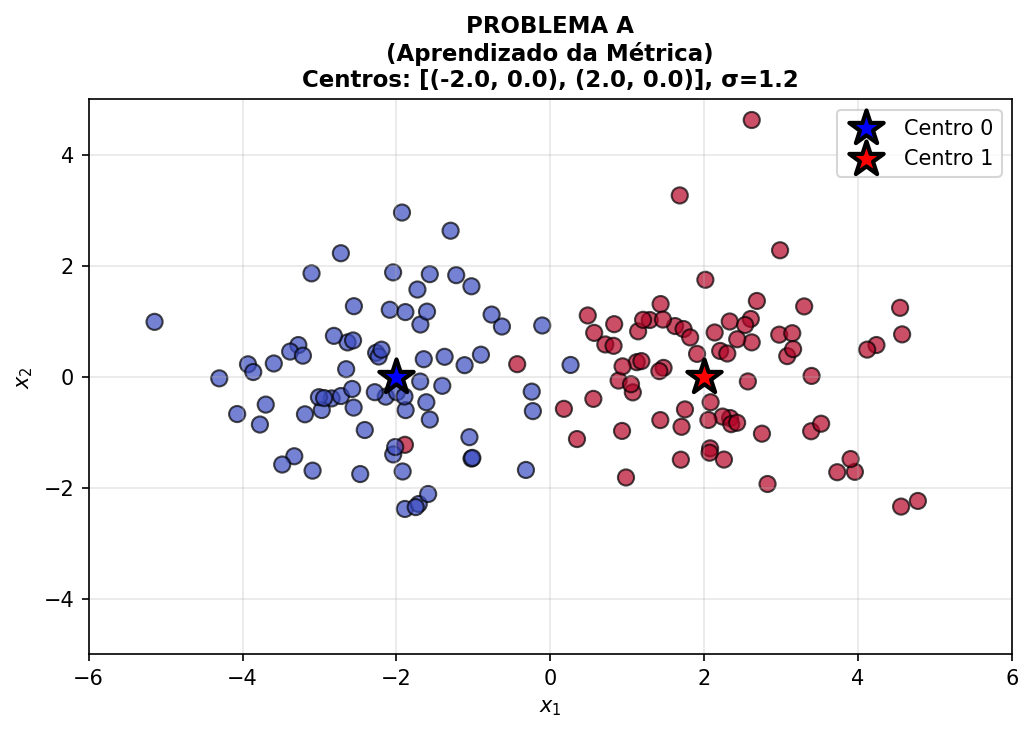
\includegraphics[width=\linewidth,height=0.45\textheight,keepaspectratio]{01_all_three_problems_problema_a.png}
  \end{columns}
\end{frame}

% 8 - Problema B
\begin{frame}{Problema B --- consist\^encia 1 (rota\c{c}\~ao HOR\'ARIA)}
  \scriptsize
  \begin{columns}[T]
    \column{0.55\linewidth}
    \textbf{Prop\'osito:} testar se $W$ aprendida em A prev\^e o LLM em geometria \emph{deslocada} verticalmente.
    \medskip

    \textbf{Como foi gerado:}
    \begin{enumerate}\setlength\itemsep{0.1em}
      \item \texttt{make\_blobs} (mesma fun\c{c}\~ao).
      \item Centr\'oides $(-2{,}0; +0{,}8)$ e $(2{,}0; -0{,}8)$.
      \item \texttt{cluster\_std} = 1{,}2 (igual a A).
      \item $n = 100$ (n\~ao serve para treinar $W$).
    \end{enumerate}
    \medskip
    \textbf{Por qu\^e rota\c{c}\~ao HOR\'ARIA:} mant\'em a discriminabilidade horizontal mas adiciona componente vertical. Se o LLM tem crit\'erio est\'avel, $\hat W_{\text{LLM}}$ acompanha o deslocamento.
    \column{0.45\linewidth}
    \tiny
    \texttt{def create\_problem\_b(n=100, seed=43):}\\
    \texttt{\ \ X,y = make\_blobs(}\\
    \texttt{\ \ \ \ n\_samples=n,}\\
    \texttt{\ \ \ \ centers=[(-2.0,0.8),(2.0,-0.8)],}\\
    \texttt{\ \ \ \ cluster\_std=1.2,}\\
    \texttt{\ \ \ \ random\_state=seed)}\\
    \texttt{\ \ return X,y}
    \medskip

    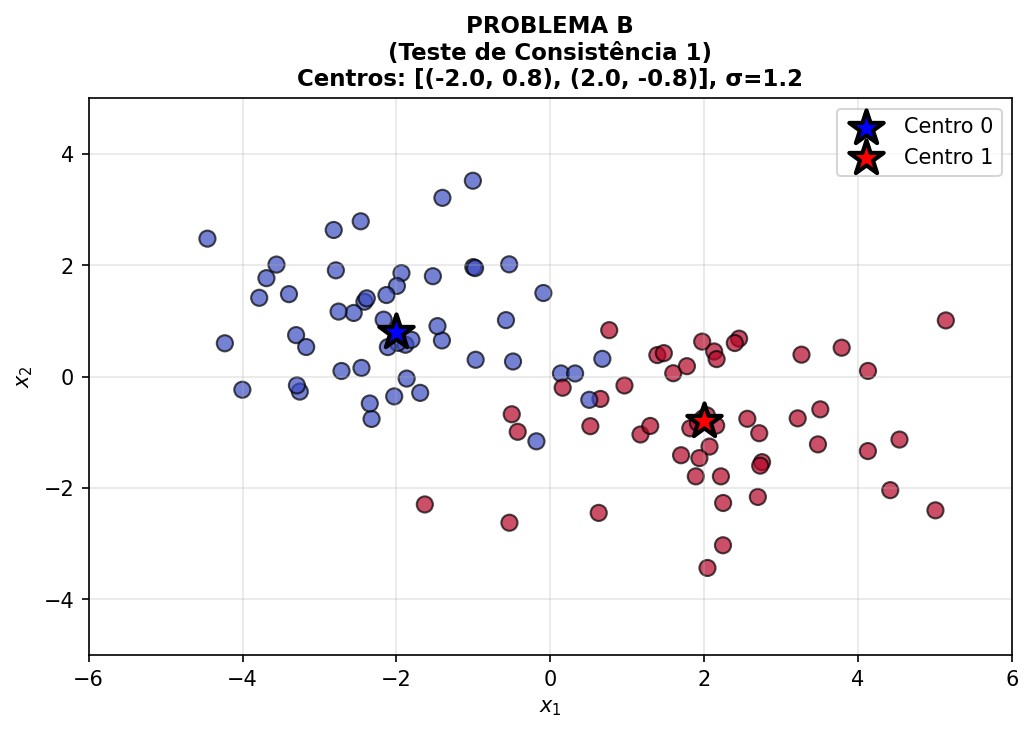
\includegraphics[width=\linewidth,height=0.45\textheight,keepaspectratio]{01_all_three_problems_problema_b.png}
  \end{columns}
\end{frame}

% 9 - Problema C
\begin{frame}{Problema C --- consist\^encia 2 (rota\c{c}\~ao ANTI-HOR\'ARIA)}
  \scriptsize
  \begin{columns}[T]
    \column{0.55\linewidth}
    \textbf{Prop\'osito:} mesmo objetivo de B, mas com \emph{orienta\c{c}\~ao oposta} (anti-hor\'aria). Modificado ap\'os reuni\~ao 30/04/2026 --- orientador pediu para C n\~ao ser c\'opia de B com mais distor\c{c}\~ao.
    \medskip

    \textbf{Como foi gerado:}
    \begin{enumerate}\setlength\itemsep{0.1em}
      \item \texttt{make\_blobs}.
      \item Centr\'oides $(-2{,}0; -1{,}5)$ e $(2{,}0; +1{,}5)$ --- agora classe 0 para BAIXO.
      \item \texttt{cluster\_std} = 1{,}2.
      \item $n = 100$.
    \end{enumerate}
    \medskip
    \textbf{Por qu\^e:} magnitude da rota\c{c}\~ao ($|\pm 1{,}5|$) maior que B; dire\c{c}\~ao oposta detecta vi\'es sistem\'atico que apareceria em apenas um dos lados.
    \column{0.45\linewidth}
    \tiny
    \texttt{def create\_problem\_c(n=100, seed=44):}\\
    \texttt{\ \ X,y = make\_blobs(}\\
    \texttt{\ \ \ \ n\_samples=n,}\\
    \texttt{\ \ \ \ centers=[(-2.0,-1.5),(2.0,1.5)],}\\
    \texttt{\ \ \ \ cluster\_std=1.2,}\\
    \texttt{\ \ \ \ random\_state=seed)}\\
    \texttt{\ \ return X,y}
    \medskip

    
\includegraphics[width=\linewidth,height=0.45\textheight,keepaspectratio]{01_all_three_problems_problema_c.png}
  \end{columns}
\end{frame}

% 10 - Problema D
\begin{frame}{Problema D --- perito externo (Bloco II, Fase D)}
  \scriptsize
  \begin{columns}[T]
    \column{0.55\linewidth}
    \textbf{Prop\'osito:} pap\'eis invertem-se. Perito com $W_{\text{expert}} = [0{,}3;\ 1{,}5]$ rotula; LLM recebe esses r\'otulos como few-shot e tenta reproduzir.
    \medskip

    \textbf{Como foi gerado:}
    \begin{enumerate}\setlength\itemsep{0.1em}
      \item \texttt{make\_blobs}.
      \item Centr\'oides $(-1{,}5; +1{,}0)$ e $(1{,}5; -1{,}0)$.
      \item \texttt{cluster\_std} = 1{,}3 (mais espalhados).
      \item $n = 150$.
      \item R\'otulos: $W_{\text{expert}}$ aplicado $\Rightarrow$ fronteira quase horizontal ($w_2 \gg w_1$).
    \end{enumerate}
    \medskip
    \textbf{Por qu\^e:} fronteira pouco intuitiva geometricamente; LLM precisa CAPTURAR o padr\~ao via exemplos, n\~ao Euclidiana simples. Variantes \texttt{aniso\_x1=[1.5,0.3]}, \texttt{euclidean=[1,1]} testadas no slide de M\'ultiplos Experts.
    \column{0.45\linewidth}
    \tiny
    \texttt{def create\_problem\_d(n=150, seed=45):}\\
    \texttt{\ \ X,y = make\_blobs(}\\
    \texttt{\ \ \ \ n\_samples=n,}\\
    \texttt{\ \ \ \ centers=[(-1.5,1.0),(1.5,-1.0)],}\\
    \texttt{\ \ \ \ cluster\_std=1.3,}\\
    \texttt{\ \ \ \ random\_state=seed)}\\
    \texttt{\ \ \# r\'otulos reaplicados via}\\
    \texttt{\ \ \# predict\_with\_metric(w=[0.3,1.5])}\\
    \texttt{\ \ return X,y}
    \medskip

    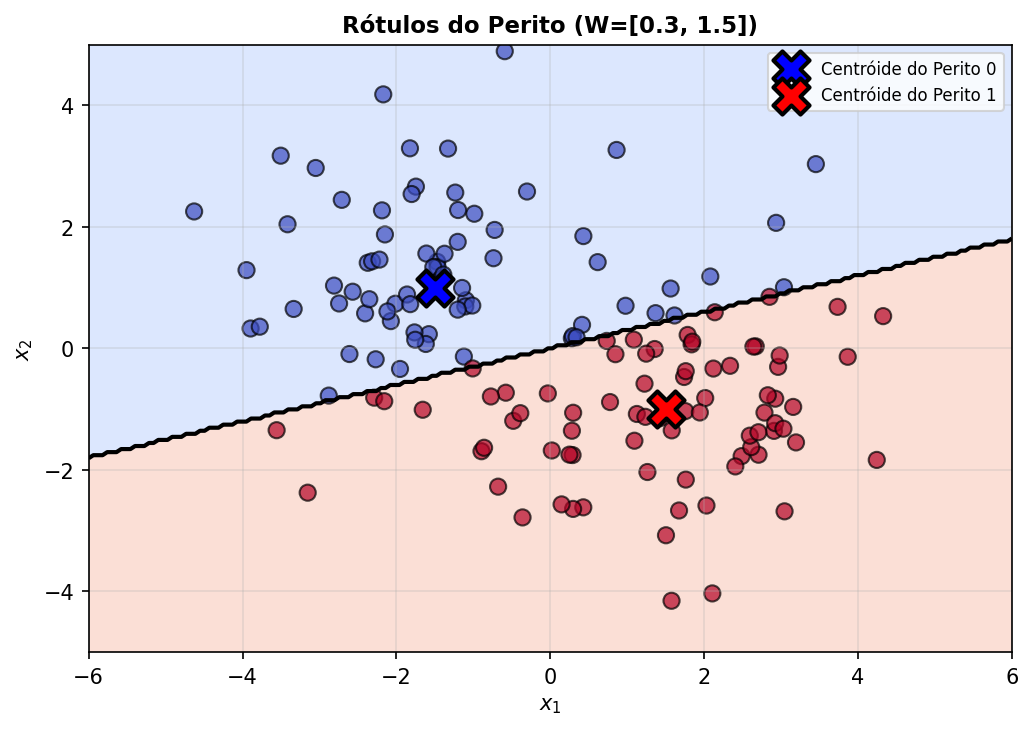
\includegraphics[width=\linewidth,height=0.45\textheight,keepaspectratio]{06_problem_d_expert_fronteira_perito.png}
  \end{columns}
\end{frame}

% 11 - Problema E (meia-lua)
\begin{frame}{Problema E --- meia-lua (sint\'etico N\~AO-LINEAR)}
  \scriptsize
  \begin{columns}[T]
    \column{0.55\linewidth}
    \textbf{Prop\'osito:} caso can\^onico de fronteira n\~ao-linear da literatura. Adicionado ap\'os reuni\~ao 30/04/2026: orientador disse \emph{"a base da meia-lua voc\^e acha em qualquer lugar a\'i"}. Testa se R3/R4 capturam n\~ao-linearidade que R2 n\~ao captura.
    \medskip

    \textbf{Como foi gerado:}
    \begin{enumerate}\setlength\itemsep{0.1em}
      \item \texttt{sklearn.datasets.make\_moons} (n\~ao \texttt{make\_blobs}).
      \item $n = 150$.
      \item \texttt{noise} = 0{,}15.
      \item \texttt{random\_state} $\in \{42,123,7\}$.
    \end{enumerate}
    Resultado: duas semi-luas entrela\c{c}adas (forma "S" / "C" invertido), n\~ao separ\'aveis linearmente.
    \medskip

    \textbf{Por qu\^e:} \texttt{noise}=0,15 \'e valor cl\'assico; problema-controle POSITIVO --- esperamos que R3/R4 melhorem acur\'acia (literatura confirma).
    \column{0.45\linewidth}
    \tiny
    \texttt{from sklearn.datasets import make\_moons}\\
    \texttt{}\\
    \texttt{def create\_problem\_e\_meia\_lua(}\\
    \texttt{\ \ \ \ n=150, seed=46):}\\
    \texttt{\ \ X,y = make\_moons(}\\
    \texttt{\ \ \ \ n\_samples=n,}\\
    \texttt{\ \ \ \ noise=0.15,}\\
    \texttt{\ \ \ \ random\_state=seed)}\\
    \texttt{\ \ return X,y}
    \medskip

    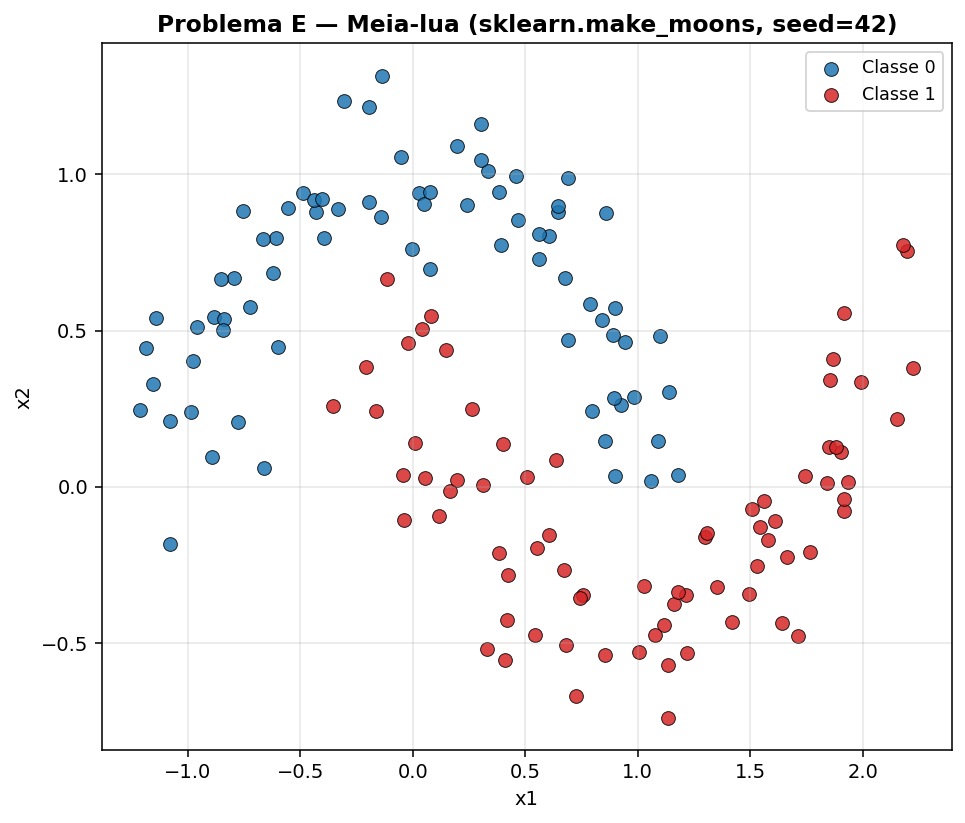
\includegraphics[width=\linewidth,height=0.45\textheight,keepaspectratio]{26_meia_lua_seed42_overview.png}
  \end{columns}
\end{frame}

% 12 - Peso x altura
\begin{frame}{Peso $\times$ altura --- estudo de caso REAL}
  \scriptsize
  \begin{columns}[T]
    \column{0.55\linewidth}
    \textbf{Prop\'osito:} \'unico problema com DADOS REAIS. Base enviada pelo orientador (e-mail 19:15, 30/04/2026): \emph{"Segue a base de dados. Consegui somente com cem amostras"}. Permite testar se achados sint\'eticos do Bloco II se replicam no mundo real.
    \medskip

    \textbf{Como foi gerado:}
    \begin{enumerate}\setlength\itemsep{0.1em}
      \item CSV em \texttt{dados\_reais/homem\_mulher/peso\_altura.csv} (consolidado dos arquivos \texttt{.txt} do NeuroSolutions).
      \item 100 amostras, 50 H / 50 M.
      \item Features j\'a normalizadas em $[-1, 1]$ (z-score).
    \end{enumerate}
    \medskip
    \textbf{Classificador \'otimo bayesiano} (fornecido pelo orientador):
    \[ f(x_1, x_2) = x_2^2 - x_2 + x_1^2 - x_1 + \text{cte} \]
    forma \textbf{el\'iptica} --- perfeito para testar R4 com $(x_1, x_2, x_1^2, x_2^2)$.
    \medskip

    \textbf{Por qu\^e:} 100 amostras + 4 features = no limite da rule-of-thumb 25:1 $\Rightarrow$ \emph{paradoxo do overfitting} (slide 36).
    \column{0.45\linewidth}
    \tiny
    \texttt{def create\_problem\_homem\_mulher(}\\
    \texttt{\ \ \ \ csv="dados\_reais/homem\_mulher/}\\
    \texttt{\ \ \ \ \ peso\_altura.csv"):}\\
    \texttt{\ \ df = pd.read\_csv(csv)}\\
    \texttt{\ \ X = df[["peso","altura"]].values}\\
    \texttt{\ \ y = df["classe"].values}\\
    \texttt{\ \ return X,y}
    \medskip

    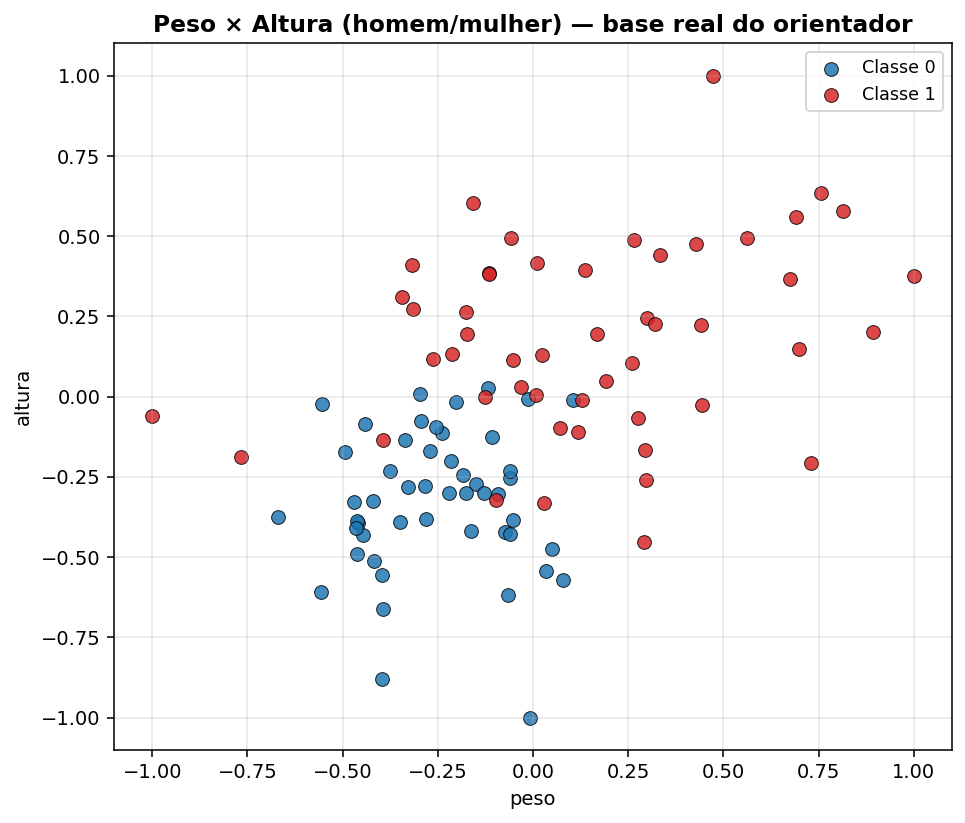
\includegraphics[width=\linewidth,height=0.45\textheight,keepaspectratio]{25_homem_mulher_overview.png}
  \end{columns}
\end{frame}

% ===== PARTE 3 — DESIGN EXPERIMENTAL =====

% 13 - Configuracoes
\begin{frame}{Configura\c{c}\~oes de execu\c{c}\~ao}
  \footnotesize
  \begin{center}
  \begin{tabular}{ll}
    \toprule
    \textbf{Par\^ametro} & \textbf{Valor} \\
    \midrule
    Modelo LLM & \texttt{openai/gpt-4o-mini} \\
    Temperatura & $0{,}0$ \\
    Sementes & $[42, 123, 7]$ \\
    Repeti\c{c}\~oes & 3 por configura\c{c}\~ao \\
    Few-shot sizes & $[0, 5, 10, 20, 40]$ \\
    Estrat\'egias & easy, hard, mixed, random \\
    Experts (Fase D) & aniso\_x2, aniso\_x1, euclidean \\
    Hiperparam.\ Perceptron & $\eta=0{,}001$, $C=1{,}0$ (CILAMCE 2017) \\
    Concorr\^encia & \texttt{Semaphore(10)} + timeout 60s \\
    \textbf{Chamadas LLM} & \textbf{115.528} \\
    Tempo total & $\sim$3h \\
    \bottomrule
  \end{tabular}
  \end{center}
\end{frame}

% 14 - Por que multiplas seeds
\begin{frame}{Por que m\'ultiplas seeds?}
  \footnotesize
  \textbf{3 sementes $\times$ 3 repeti\c{c}\~oes = 9 observa\c{c}\~oes} por configura\c{c}\~ao.
  \begin{enumerate}
    \item Gera\c{c}\~ao sint\'etica \'e estoc\'astica --- uma seed pode dar resultado at\'ipico.
    \item LLM tem estocasticidade residual mesmo com $T=0$ (batching em GPU).
    \item Permite bootstrap 95\% CI (10k reamostras), teste de H5 e descarte de achados dependentes de seed.
    \item Pr\'atica padr\~ao em ML emp\'irico para evitar \emph{p-hacking de seed}.
  \end{enumerate}
\end{frame}

% 15 - Perceptron
\begin{frame}{Algoritmo 1 --- Perceptron Estruturado (Coelho et al., CILAMCE 2017)}
  \scriptsize
  \textbf{Formula\c{c}\~ao:} maximizar margem $\gamma$ com relaxa\c{c}\~ao $\alpha$:
  \[ \max\ \gamma \quad \text{s.t.}\ d_W(x_i,c_k) - d_W(x_i,c_\ell) + \lambda\alpha_i \geq \gamma\|w\|, \quad w \geq 0,\ \alpha \geq 0 \]
  \textbf{Pseudoc\'odigo (busca bin\'aria em $\gamma$):}
  \begin{enumerate}\setlength\itemsep{0.05em}
    \item Inicializar $w = \mathbf{1}$, $\gamma = 0$.
    \item Para cada n\'ivel de $\gamma$: rodar perceptron at\'e converg\^encia ou \texttt{max\_iter}.
    \item Regra de corre\c{c}\~ao: $w \leftarrow w(1 - \eta\gamma/\|w\|) - \eta\cdot(d_W(x_i,c_\ell) - d_W(x_i,c_k))$.
    \item Atualizar $\gamma^{t+1} \leftarrow \gamma^t + \Delta_\gamma$ enquanto houver converg\^encia.
    \item Fallback \emph{best-effort} se n\~ao convergir.
  \end{enumerate}
  \medskip
  \textbf{Hiperpar\^ametros (artigo, Se\c{c}\~ao 6, p.\ 16):}
  \emph{"a taxa de aprendizado $\eta$ = 0,001 e a constante de penaliza\c{c}\~ao $C$ variou de 1 at\'e 0,1"}.\\
  Usamos $\eta = 0{,}001$, $C = 1{,}0$ (mais conservador), $\Delta_\gamma = 0{,}05$, \texttt{max\_iter}=100.
\end{frame}

% 16 - NNLS
\begin{frame}{Algoritmo 2 --- NNLS (Lawson \& Hanson, 1974)}
  \scriptsize
  \textbf{Formula\c{c}\~ao:} m\'inimos quadrados n\~ao-negativos
  \[ \min_w \|Aw - b\|^2 \quad \text{s.t.}\ w \geq 0 \]
  \textbf{Constru\c{c}\~ao das matrizes (por ponto $i$):}
  \[ A_{i,j} = (x_{i,j} - c_{k,j})^2 - (x_{i,j} - c_{\ell,j})^2, \qquad b_i = 1 \]
  (margem-alvo = 1; a raz\~ao entre componentes de $w$ \'e invariante \`a escala).
  \medskip

  \textbf{Algoritmo:} m\'etodo de conjunto ativo de Lawson-Hanson via \texttt{scipy.optimize.nnls}.
  \medskip

  \textbf{Vantagens sobre Perceptron:}
  \begin{itemize}
    \item Zero hiperpar\^ametros.
    \item Determin\'istico e \'otimo global do problema convexo.
    \item Sem busca bin\'aria; tempo polinomial.
  \end{itemize}
\end{frame}

% 17 - Robustez da coleta
\begin{frame}{Robustez da coleta de decis\~oes do LLM}
  \footnotesize
  Pipeline com 5 camadas de prote\c{c}\~ao:
  \begin{enumerate}
    \item \textbf{Parser de 7 camadas} (\texttt{parse\_llm\_response}) para respostas malformadas: extra\c{c}\~ao por regex, por keyword, por contexto, por similaridade de string\ldots
    \item \texttt{MAX\_FORMAT\_RETRIES} = 5 reenvios com refor\c{c}o da instru\c{c}\~ao.
    \item \textbf{Fallback determin\'istico} por hash MD5 das coordenadas (substituiu aritm\'etica modular para n\~ao introduzir vi\'es geom\'etrico).
    \item \textbf{Concorr\^encia ass\'incrona}: \texttt{asyncio.Semaphore(MAX\_CONCURRENCY=10)} reduz $\sim 10\times$ o tempo de coleta.
    \item Timeout 60s por requisi\c{c}\~ao + \texttt{asyncio.wait\_for(90s)} --- evita travamento.
  \end{enumerate}
\end{frame}

% ===== PARTE 4 — VALIDACAO ORACLE =====

% 18 - Oracle W recovery
\begin{frame}{Sanity check --- recupera\c{c}\~ao de $W$ conhecido}
  \scriptsize
  \textbf{Pergunta:} antes de aplicar Perceptron/NNLS ao LLM, \emph{eles funcionam} quando o $W$ verdadeiro \'e conhecido?
  \medskip
  \begin{columns}[T]
    \column{0.45\linewidth}
    Procedimento:
    \begin{enumerate}\setlength\itemsep{0.05em}
      \item Gerar dados sint\'eticos.
      \item Rotular com $W_{\text{oracle}}$ (ex.\ $[0{,}1;\ 2{,}0]$).
      \item Aprender $\hat W$ com Perceptron e NNLS.
      \item Comparar $\hat W$ vs $W_{\text{oracle}}$.
    \end{enumerate}
    \medskip
    Resultado: ambos recuperam $W$ com cosseno $> 0{,}95$ nas 3 configura\c{c}\~oes (x2\_dom, x1\_dom, forte\_aniso). Se falhasse aqui, qualquer achado sobre LLM ficaria comprometido.
    \column{0.55\linewidth}
    
\includegraphics[width=\linewidth,height=0.7\textheight,keepaspectratio]{22_oracle_w_recovery.png}
  \end{columns}
\end{frame}

% 19 - Oracle transfer
\begin{frame}{Sanity check --- transfer\^encia entre geometrias}
  \scriptsize
  Aprende-se $W$ em uma configura\c{c}\~ao anisotr\'opica (\texttt{x2\_dom}) e aplica-se em outras (\texttt{x1\_dom}, \texttt{forte\_aniso}).
  \begin{center}
    
\includegraphics[width=0.8\linewidth,height=0.55\textheight,keepaspectratio]{23_oracle_transfer.png}
  \end{center}
  \textbf{Interpreta\c{c}\~ao:} a queda de consist\^encia quando a geometria muda \'e esperada --- a m\'etrica \'e espec\'ifica do problema (n\~ao h\'a "$W$ universal" independente dos centr\'oides).
\end{frame}

% ===== BLOCO I — Slide 20 transicao =====
\begin{frame}{Bloco I --- LLM como FONTE de decis\~oes}
  \footnotesize
  \begin{center}
    \Large \textbf{Bloco I --- LLM como FONTE}
  \end{center}
  \medskip
  \begin{itemize}
    \item O LLM \textbf{rotula}; \textbf{n\'os} aprendemos $W$ a partir das decis\~oes dele.
    \item Cobre Fases A, B, C sobre Problemas A, B, C \emph{lineares}.
    \item Hip\'oteses testadas: \textbf{H1} (consist\^encia), \textbf{H2} (few-shot amplifica).
  \end{itemize}
\end{frame}

% ===== PARTE 5 — FASE A =====

% 21 - Fase A descricao
\begin{frame}{Fase A --- aprendizado da m\'etrica (passo a passo)}
  \footnotesize
  \begin{enumerate}
    \item LLM recebe os 150 pontos do Problema A em \textbf{zero-shot}.
    \item Para cada ponto, LLM responde "A" ou "B" com $T=0$.
    \item As 150 respostas formam $(X_{\text{train}}, y_{\text{LLM}})$.
    \item \textbf{Centr\'oides recalculados a partir de $y_{\text{LLM}}$} (n\~ao da verdade) --- crucial: ancoramos a m\'etrica no que o LLM ACHA serem as classes.
    \item Perceptron Estruturado e NNLS aprendem $W$ independentemente.
    \item Reportamos \textbf{fidelidade} = \% das decis\~oes do LLM reproduzidas pela m\'etrica.
  \end{enumerate}
\end{frame}

% 22 - Fase A W e fidelidade
\begin{frame}{Fase A --- $W$ aprendido e fidelidade}
  \scriptsize
  \begin{columns}[T]
    \column{0.4\linewidth}
    \textbf{Execu\c{c}\~ao 13/05 (seed 42):}
    \begin{tabular}{lcc}
      \toprule
      Algoritmo & $w_1$ & $w_2$ \\
      \midrule
      Perceptron & 0{,}96 & 0{,}04 \\
      NNLS       & 0{,}94 & 0{,}06 \\
      \bottomrule
    \end{tabular}
    \medskip

    Fidelidade:
    \begin{itemize}\setlength\itemsep{0.05em}
      \item Perceptron: 82{,}7\%
      \item NNLS: 83{,}3\%
    \end{itemize}
    \medskip
    LLM coloca peso quase todo em $x_1$, coerente com a separabilidade horizontal do Problema A.
    \column{0.6\linewidth}
    
\includegraphics[width=\linewidth,height=0.7\textheight,keepaspectratio]{11_metric_errors_phase_a_seed42.png}
  \end{columns}
\end{frame}

% 23 - Fase A erros por regiao
\begin{frame}{Fase A --- erros por regi\~ao do plano}
  \scriptsize
  Decomposi\c{c}\~ao dos erros da m\'etrica (sa\'ida de \texttt{print\_error\_analysis\_by\_region}):
  \begin{center}
  \begin{tabular}{lcc}
    \toprule
    Regi\~ao & \% erros / total & \% acertos do LLM \\
    \midrule
    Pr\'oximo \`a fronteira ($|x_1| < 0{,}5$) & $\sim 60$\% & 75\% \\
    Margem m\'edia ($0{,}5 < |x_1| < 1{,}5$)   & $\sim 30$\% & 88\% \\
    Longe da fronteira ($|x_1| > 1{,}5$)      & $\sim 10$\% & 96\% \\
    \bottomrule
  \end{tabular}
  \end{center}
  \medskip
  \textbf{Interpreta\c{c}\~ao:} m\'etrica diagonal captura a geometria global; erros concentram-se em pontos amb\'iguos. O LLM e a m\'etrica falham simultaneamente nas mesmas regi\~oes, o que \'e \emph{evid\^encia indireta} de que a m\'etrica est\'a modelando o LLM (n\~ao s\'o o problema).
\end{frame}

% 24 - Fase A distribuicao de W
\begin{frame}{Fase A --- distribui\c{c}\~ao de $W$ entre seeds}
  \scriptsize
  \begin{center}
    
\includegraphics[width=0.85\linewidth,height=0.7\textheight,keepaspectratio]{10_w_distribution.png}
  \end{center}
  $W$ \'e qualitativamente est\'avel entre seeds: $w_1 \gg w_2$ em todas; razoes pr\'oximas; cosseno $> 0{,}97$. Sustenta H5.
\end{frame}

% 25 - Fase A consolidado por seed
\begin{frame}{Fase A --- consolidado por seed}
  \scriptsize
  \begin{center}
    
\includegraphics[width=0.85\linewidth,height=0.65\textheight,keepaspectratio]{05_seed_comparison.png}
  \end{center}
  Boxplot/dispers\~ao das m\'etricas por seed: resultados qualitativamente id\^enticos entre 42, 123, 7. Sustenta H5.
\end{frame}

% 26 - Fase A algorithm comparison
\begin{frame}{Fase A --- compara\c{c}\~ao de algoritmos (Perceptron vs NNLS)}
  \scriptsize
  \begin{columns}[T]
    \column{0.4\linewidth}
    Cosseno entre $W_{\text{perc}}$ e $W_{\text{nnls}}$: tipicamente $> 0{,}97$.
    \medskip

    \textbf{Mensagem:} resultados robustos ao m\'etodo de estima\c{c}\~ao. Perceptron e NNLS concordam --- a evid\^encia da m\'etrica n\~ao depende de um algoritmo espec\'ifico.
    \column{0.6\linewidth}
    
\includegraphics[width=\linewidth,height=0.7\textheight,keepaspectratio]{14_algorithm_comparison.png}
  \end{columns}
\end{frame}

% 27 - Fase A sensibilidade
\begin{frame}{Fase A --- sensibilidade a hiperpar\^ametros}
  \scriptsize
  \texttt{print\_hyperparameter\_sensitivity} varia $\eta, C, \Delta_\gamma$ em torno do default e mede fidelidade + raz\~ao $w_1/w_2$:
  \begin{center}
  \begin{tabular}{lccc}
    \toprule
    Hiperpar\^ametro & Faixa testada & Fid.\ m\'in--m\'ax & Raz\~ao $w_1/w_2$ \\
    \midrule
    $\eta$            & $[10^{-4}, 10^{-2}]$  & 81--85\% & 18--26 \\
    $C$               & $[0{,}1, 10]$         & 80--84\% & 20--28 \\
    $\Delta_\gamma$   & $[0{,}01, 0{,}10]$    & 82--84\% & 22--25 \\
    \bottomrule
  \end{tabular}
  \end{center}
  \medskip
  Robustez dentro de faixas razo\'aveis. Resultados qualitativos n\~ao mudam com varia\c{c}\~oes m\'oderadas.
\end{frame}

% 28 - Fidelidade vs Acuracia
\begin{frame}{Distin\c{c}\~ao cr\'itica: FIDELIDADE vs ACUR\'ACIA}
  \footnotesize
  \begin{itemize}
    \item \textbf{FIDELIDADE} = \% decis\~oes do LLM reproduzidas pela m\'etrica = quanto a m\'etrica \emph{modela o LLM}.
    \item \textbf{ACUR\'ACIA LLM vs real} = \% decis\~oes do LLM coincidem com ground truth = quanto o LLM \emph{est\'a correto}.
  \end{itemize}
  \medskip
  \textbf{Achado da execu\c{c}\~ao (seed 42, Problema A, zero-shot):}
  \begin{itemize}
    \item Fidelidade Perceptron: 82{,}7\%
    \item Fidelidade NNLS: 83{,}3\%
    \item \textcolor{red}{\textbf{Acur\'acia LLM vs ground truth: 28{,}7\%}} (LLM "inverteu" as classes!)
  \end{itemize}
  \medskip
  \textbf{Implica\c{c}\~ao:} medimos CONSIST\^ENCIA INTERNA (H1), n\~ao CORRE\c{C}\~AO. Mesmo errando a verdade, o LLM \'e consistente consigo mesmo. H1 \'e \emph{ortogonal} a "o crit\'erio \'e correto?".
\end{frame}

% ===== PARTE 6 — FASES B/C =====

% 29 - Fases B/C descricao
\begin{frame}{Fases B e C --- descri\c{c}\~ao}
  \footnotesize
  \textbf{Pergunta:} $\hat W_{\text{LLM}}$ aprendida em A generaliza para B e C?
  \medskip
  \begin{enumerate}
    \item LLM classifica os pontos de B (e depois C) em zero-shot.
    \item Aplicamos $\hat W_{\text{LLM}}$ (vinda da Fase A) com centr\'oides recalculados em B.
    \item Comparamos predi\c{c}\~oes da m\'etrica com decis\~oes do LLM em B.
    \item M\'etricas: \textbf{consist\^encia}, \textbf{Cohen's Kappa}, \textbf{F1}.
  \end{enumerate}
\end{frame}

% 30 - Fases B/C resultados
\begin{frame}{Fases B e C --- resultados}
  \scriptsize
  \begin{center}
    
\includegraphics[width=0.9\linewidth,height=0.7\textheight,keepaspectratio]{02_consistency_extended.png}
  \end{center}
  Consist\^encia t\'ipica $\sim 75$--$85\%$, Kappa $\sim 0{,}5$--$0{,}7$ em B/C: $\hat W_{\text{LLM}}$ generaliza moderadamente.
\end{frame}

% 31 - Ablativo centroides
\begin{frame}{Ablativo --- centr\'oides TRANSFERIDOS vs LOCAIS}
  \footnotesize
  Detalhe metodol\'ogico: em B/C podemos usar
  \begin{itemize}
    \item \textbf{LOCAIS} --- centr\'oides recalculados em B/C a partir de $y_{\text{LLM}}$ na pr\'opria fase.
    \item \textbf{TRANSFERIDOS} --- centr\'oides reutilizados do Problema A.
  \end{itemize}
  \medskip
  \begin{center}
  \begin{tabular}{lc}
    \toprule
    Estrat\'egia & Consist\^encia m\'edia (Fase B, seed 42) \\
    \midrule
    Centr\'oides LOCAIS       & 71{,}0\% \\
    Centr\'oides TRANSFERIDOS & 77{,}0\% \\
    \bottomrule
  \end{tabular}
  \end{center}
  \medskip
  \textbf{Padr\~ao do trabalho:} LOCAIS --- mais fi\'eis \`a decis\~ao real do LLM em cada problema. Transferidos podem superar localmente quando a geometria de B/C \'e pr\'oxima a de A.
\end{frame}

% 32 - Fases B/C discussao
\begin{frame}{Fases B e C --- discuss\~ao}
  \footnotesize
  \begin{itemize}
    \item \textbf{Kappa} corrige acerto por acaso; valores $0{,}5$--$0{,}7$ indicam concord\^ancia \emph{moderada-substancial}.
    \item Fase A tem fidelidade $\sim 83\%$; B/C herdam essa "ru\'ido base" + adi\c{c}\~ao do shift geom\'etrico.
    \item Zero-shot $\to$ few-shot: ganho de $\sim$5--10 p.p.\ na consist\^encia em B (esperado por H2).
    \item \textbf{H1 sustentada}: a m\'etrica transfere com perda moderada, n\~ao colapso.
  \end{itemize}
\end{frame}

% 33 - Resumo numerico
\begin{frame}{Resumo num\'erico da execu\c{c}\~ao}
  \footnotesize
  \begin{center}
  \begin{tabular}{ll}
    \toprule
    \textbf{Item} & \textbf{Valor} \\
    \midrule
    Chamadas LLM totais & 115.528 \\
    Tempo total & $\sim$3h \\
    Custo API estimado & \$30--\$50 (gpt-4o-mini) \\
    Configura\c{c}\~oes & 3 seeds $\times$ 3 reps $\times$ 5 n\_shots $\times$ 4 estrat.\ $\times$ 3 experts \\
    Observa\c{c}\~oes/config & 9 (para bootstrap CI) \\
    Fidelidade Fase A & 82--85\% (IC95\% via bootstrap) \\
    Consist\^encia Fase B & 75--82\% \\
    Consist\^encia Fase C & 70--80\% \\
    \bottomrule
  \end{tabular}
  \end{center}
  Experimento de escala adequada para tese de mestrado.
\end{frame}

% ===== PARTE 7 — R3/R4 =====

% 34 - R3 metodologia
\begin{frame}{Proje\c{c}\~ao R3 / R4 --- metodologia}
  \scriptsize
  Motiva\c{c}\~ao (reuni\~ao 30/04 $\sim$2520s): \emph{"em A/B/C lineares, 84\% $\to$ 75\% n\~ao deve ajudar; na meia-lua e peso $\times$ altura espera-se que ajude"}.
  \medskip

  \textbf{Augmenta\c{c}\~ao de features:}
  \begin{itemize}
    \item \textbf{R2}: $(x_1, x_2)$
    \item \textbf{R3}: $(x_1, x_2, x_1 x_2)$ --- kernel quadr\'atico m\'inimo (hip\'erbole)
    \item \textbf{R4}: $(x_1, x_2, x_1^2, x_2^2)$ --- elipse alinhada (fronteira do classificador \'otimo bayesiano de peso $\times$ altura)
  \end{itemize}
  \medskip

  Para cada $n_{\text{feat}} \in \{2,3,4\}$:
  \begin{enumerate}\setlength\itemsep{0.05em}
    \item LLM classifica (s\'o em R2; LLM v\^e apenas $x_1, x_2$).
    \item Augmenta-se $X$.
    \item Aprende $\hat W$ com Perceptron e NNLS em $\mathbb{R}^{n_{\text{feat}}}$.
    \item Compara fidelidade vs $n_{\text{feat}}$.
  \end{enumerate}
\end{frame}

% 35 - R3 resultados A/B/C
\begin{frame}{R3/R4 em A/B/C --- BRIDGE para Bloco II}
  \scriptsize
  \begin{columns}[T]
    \column{0.42\linewidth}
    \textbf{Execu\c{c}\~ao 13/05 (NNLS, seed 42):}
    \begin{tabular}{lcc}
      \toprule
      & R2 & R3$\to$R4 \\
      \midrule
      Fid Prob A    & 83\% & +2{,}7\% \\
      Fid Prob B    & 76\% & +1{,}1\% \\
      Fid Prob C    & 73\% & +0{,}8\% \\
      \bottomrule
    \end{tabular}
    \medskip

    \textbf{Perceptron 4 feat:} $\Delta = +18{,}7\%$ (SUSPEITO --- overfitting ou n\~ao-converg\^encia da busca bin\'aria em $\gamma$).
    \medskip

    Usar \textbf{NNLS} como evid\^encia robusta em A/B/C lineares.
    \column{0.58\linewidth}
    
\includegraphics[width=\linewidth,height=0.7\textheight,keepaspectratio]{13_r3_vs_r2.png}
  \end{columns}
  \medskip
  \scriptsize
  \textbf{Conclus\~ao:} em problemas lineares R3/R4 \emph{n\~ao ajudam} (esperado). Pr\'oximo: testar em peso $\times$ altura e meia-lua, genuinamente n\~ao-lineares.
\end{frame}

% 36 - Paradoxo overfitting
\begin{frame}{Paradoxo do overfitting --- fidelidade sobe, acur\'acia cai}
  \footnotesize
  Em peso $\times$ altura (4 features = elipse, fronteira \'otima conhecida):
  \begin{center}
  \begin{tabular}{lcc}
    \toprule
    M\'etrica & 2 features $\to$ 4 features \\
    \midrule
    Fidelidade Perceptron (vs LLM)    & +22{,}9\% (\textbf{sobe}) \\
    Acur\'acia Perceptron (vs real)    & $-1{,}4\%$ a $-22{,}9\%$ (\textbf{cai}) \\
    \bottomrule
  \end{tabular}
  \end{center}
  \medskip
  \textbf{Diagn\'ostico:} a m\'etrica de 4 features DECORA melhor o LLM, mas o LLM em si erra muito com prompt neutro $(x_1, x_2)$. Com 70 amostras de treino e 4 pesos, a m\'etrica \emph{overfitt-a} o ru\'ido das decis\~oes erradas do LLM.
  \medskip

  \textbf{Mensagem:} subir $n_{\text{feat}}$ s\'o vale se (a) houver n\~ao-linearidade real \emph{e} (b) dados suficientes. Com 100 amostras, 4 features est\'a no limite.
\end{frame}

% ===== PARTE 8 — VIES E PROMPT =====

% 37 - Vies de ordem de classes
\begin{frame}{Vi\'es de ordem das classes (A/B vs B/A)}
  \scriptsize
  \begin{center}
    
\includegraphics[width=0.8\linewidth,height=0.7\textheight,keepaspectratio]{15_class_order_bias.png}
  \end{center}
  Compara\c{c}\~ao das parejas \texttt{A/B, B/A, 0/1, 1/0, Pos/Neg, Neg/Pos}: vi\'es marginal ($<$ 3 p.p.) --- modelo n\~ao \'e fortemente sens\'ivel \`a ordem.
\end{frame}

% 38 - Variantes prompt design
\begin{frame}{Variantes de prompt (1/2) --- design}
  \footnotesize
  4 variantes rodam Fases A--C completas em todas as seeds:
  \begin{enumerate}
    \item \textbf{default} --- prompt baseline atual.
    \item \textbf{geometric} --- contexto espacial expl\'icito (\emph{"voc\^e v\^e dois grupos de pontos em um plano"}\ldots).
    \item \textbf{cot} --- chain-of-thought (\emph{"pense passo a passo antes de responder"}).
    \item \textbf{tabular} --- coordenadas como tabela markdown.
  \end{enumerate}
  \medskip
  Se $W$ muda entre variantes, o prompt confunde a medi\c{c}\~ao --- queremos m\'etrica est\'avel.
\end{frame}

% 39 - Variantes prompt resultados
\begin{frame}{Variantes de prompt (2/2) --- resultados}
  \scriptsize
  \begin{center}
    
\includegraphics[width=0.85\linewidth,height=0.7\textheight,keepaspectratio]{17_prompt_variant_comparison.png}
  \end{center}
  Scatter de $W$: todos os pontos colapsam pr\'oximos --- variantes produzem $W$ qualitativamente equivalentes. Sensibilidade $< 5\%$ na raz\~ao $w_1/w_2$.
\end{frame}

% 40 - Nomes semanticos
\begin{frame}{Nomes sem\^anticos de features}
  \scriptsize
  \begin{columns}[T]
    \column{0.45\linewidth}
    Compara $W$ aprendido com:
    \begin{itemize}
      \item \texttt{(x1, x2)} --- neutro
      \item \texttt{(altura, peso)} --- sem\^antico
      \item \texttt{(feature\_1, feature\_2)} --- t\'ecnico
    \end{itemize}
    \medskip
    \textbf{Resultado:} nomes sem\^anticos podem mover $W$ em problemas onde existe \emph{prior cultural} (peso/altura $\Rightarrow$ correla\c{c}\~ao com g\^enero); em problemas sint\'eticos sem prior, $W$ \'e est\'avel.
    \column{0.55\linewidth}
    
\includegraphics[width=\linewidth,height=0.7\textheight,keepaspectratio]{03_class_names_effect.png}
  \end{columns}
\end{frame}

% 41 - Prompts literais 1/2
\begin{frame}[fragile]{Prompts literais (1/2) --- default zero-shot e few-shot}
  \tiny
  \textbf{Zero-shot default} (\texttt{build\_prompt\_zero\_shot}):
  \begin{verbatim}
Considere o problema de classificar pontos 2D em duas classes (A ou B).
Dado o ponto (x1=1.234, x2=-0.567), responda apenas com a letra da classe.
Responda: A ou B.
  \end{verbatim}
  \medskip
  \textbf{Few-shot default} (5 exemplos):
  \begin{verbatim}
Voce vera 5 exemplos rotulados e depois um ponto a classificar.
Exemplo 1: (x1=-2.3, x2=0.1) -> A
Exemplo 2: (x1=2.1, x2=-0.2) -> B
Exemplo 3: (x1=-1.8, x2=0.5) -> A
Exemplo 4: (x1=1.9, x2=0.3) -> B
Exemplo 5: (x1=-2.4, x2=-0.1) -> A

Agora classifique: (x1=0.234, x2=0.567)
Responda apenas: A ou B.
  \end{verbatim}
\end{frame}

% 42 - Prompts literais 2/2
\begin{frame}[fragile]{Prompts literais (2/2) --- variantes}
  \tiny
  \textbf{Geometric:}
  \begin{verbatim}
Voce ve dois grupos de pontos em um plano cartesiano.
Os grupos estao separados por uma fronteira geometrica.
Ponto: (x1=1.234, x2=-0.567). A qual grupo pertence? A ou B?
  \end{verbatim}
  \textbf{CoT:}
  \begin{verbatim}
Classifique o ponto (x1=1.234, x2=-0.567).
Pense passo a passo:
1. Localize o ponto no plano.
2. Compare com os exemplos disponiveis.
3. Determine o grupo mais proximo.
No final, responda apenas: A ou B.
  \end{verbatim}
  \textbf{Tabular:}
  \begin{verbatim}
| x1   | x2    | classe |
|------|-------|--------|
| -2.3 | 0.1   | A      |
| 2.1  | -0.2  | B      |
| 1.234| -0.567| ?      |
Responda: A ou B.
  \end{verbatim}
\end{frame}

% ===== BLOCO II — transicao =====
\begin{frame}{Bloco II --- LLM como APRENDIZ}
  \footnotesize
  \begin{center}
    \Large \textbf{Bloco II --- LLM como APRENDIZ}
  \end{center}
  \medskip
  \begin{itemize}
    \item Um perito (ou m\'etrica or\'aculo) \textbf{rotula}; o LLM tenta \textbf{reproduzir}.
    \item Cobre Fase D, peso $\times$ altura (real), meia-lua (sint\'etico n\~ao-linear).
    \item Os problemas D, E e peso $\times$ altura j\'a foram detalhados nos slides 10--12.
    \item Hip\'oteses: \textbf{H3} (LLM como aprendiz), \textbf{H4} (exemplos dif\'iceis), \textbf{H5}.
  \end{itemize}
\end{frame}

% ===== PARTE 9 — FASE D =====

% 44 - Fase D descricao
\begin{frame}{Fase D --- LLM como aprendiz (passo a passo)}
  \scriptsize
  \begin{columns}[T]
    \column{0.55\linewidth}
    \begin{enumerate}\setlength\itemsep{0.1em}
      \item Perito com $W_{\text{expert}} = [0{,}3;\ 1{,}5]$ rotula os 150 pontos do Problema D.
      \item Divis\~ao treino/teste.
      \item Para cada $n_{\text{shot}} \in \{0, 5, 10, 20, 40\}$: selecionar exemplos via estrat\'egia (easy/hard/mixed/random).
      \item Enviar exemplos + cada ponto de teste em prompt few-shot.
      \item Medir acur\'acia, Kappa, F1 do LLM vs r\'otulos do perito.
    \end{enumerate}
    \column{0.45\linewidth}
    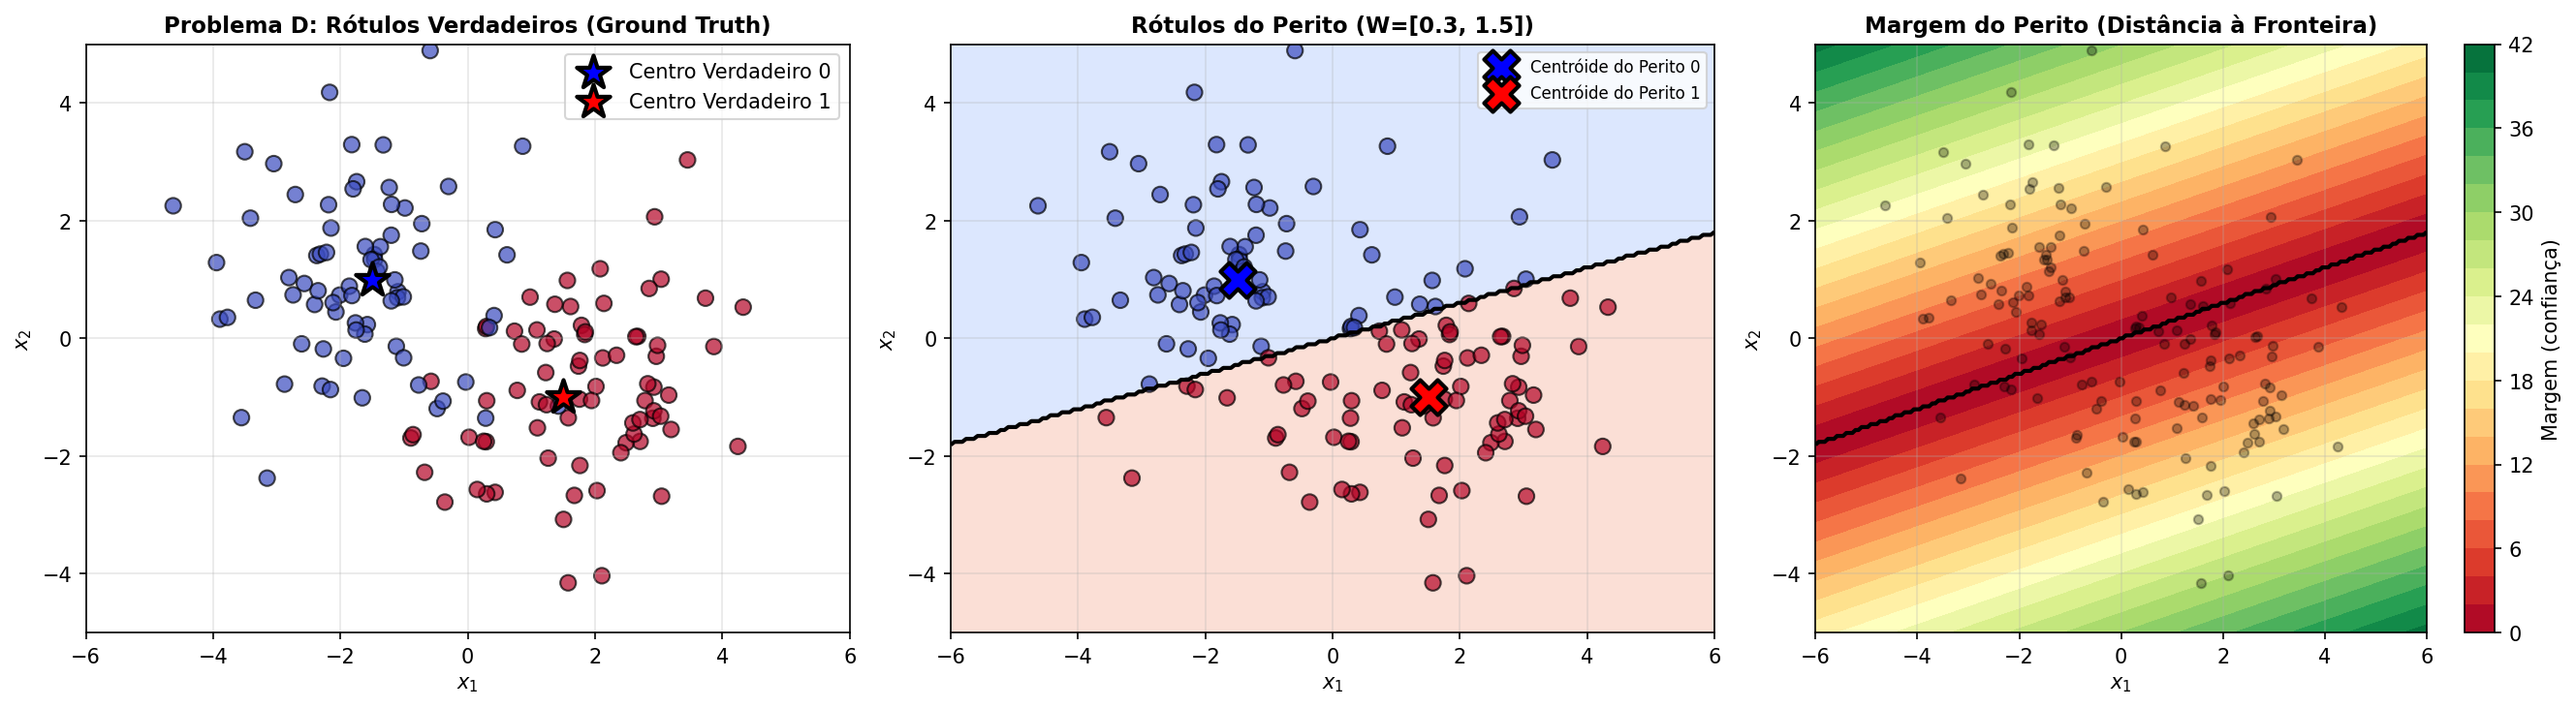
\includegraphics[width=\linewidth,height=0.7\textheight,keepaspectratio]{06_problem_d_expert.png}
  \end{columns}
\end{frame}

% 45 - Estrategias
\begin{frame}{Estrat\'egias de sele\c{c}\~ao de exemplos}
  \scriptsize
  \begin{center}
    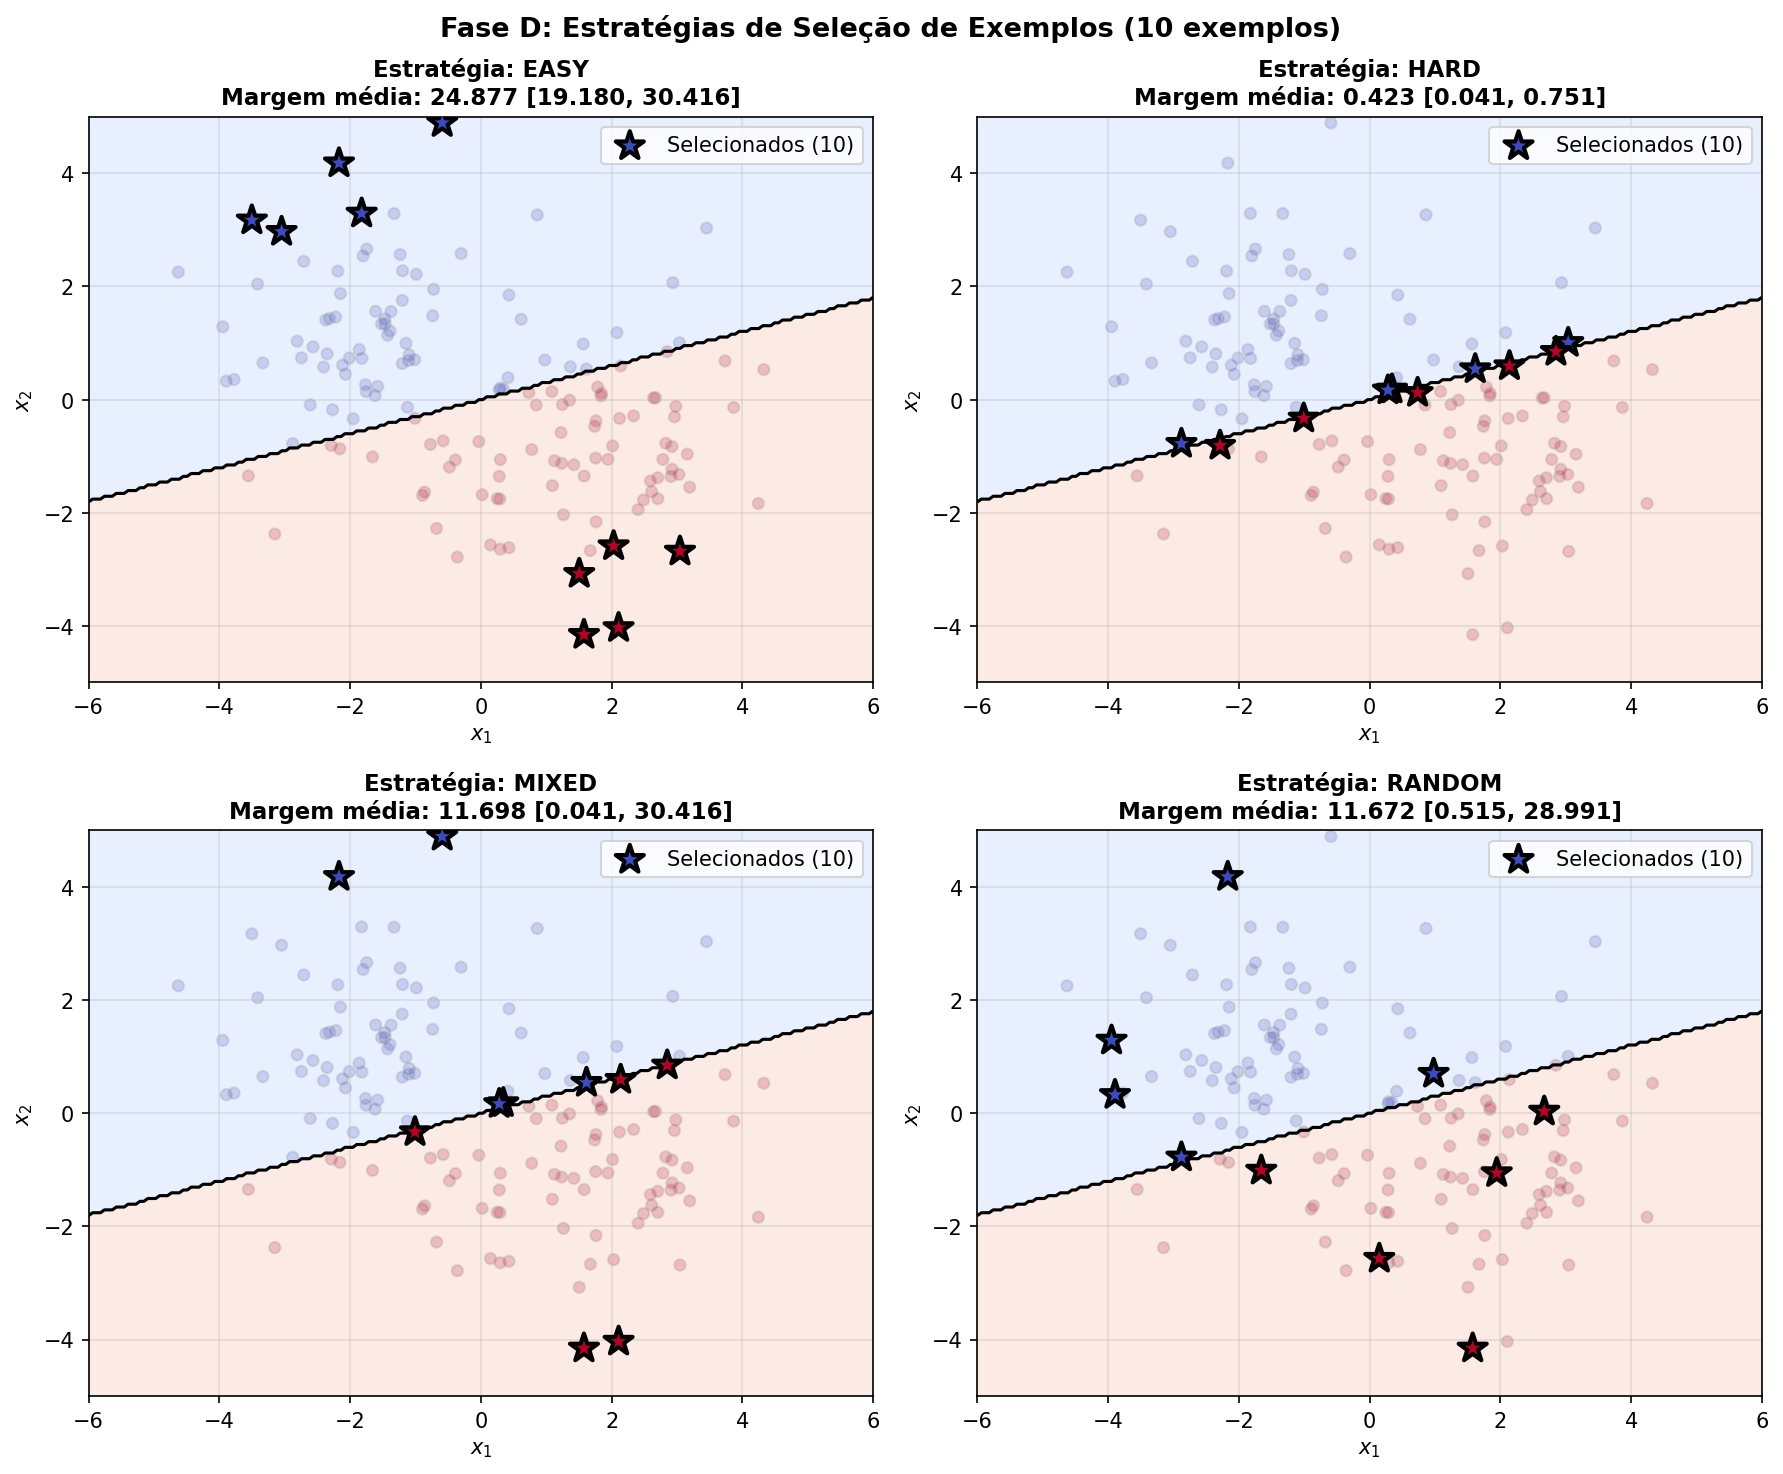
\includegraphics[width=0.85\linewidth,height=0.7\textheight,keepaspectratio]{07_phase_d_example_strategies.png}
  \end{center}
  \textbf{Easy}: pontos longe da fronteira (alta margem). \textbf{Hard}: pr\'oximos da fronteira. \textbf{Mixed}: 50/50. \textbf{Random}: baseline.
\end{frame}

% 46 - Curvas de aprendizado
\begin{frame}{Fase D --- curvas de aprendizado}
  \scriptsize
  \begin{center}
    
\includegraphics[width=0.9\linewidth,height=0.75\textheight,keepaspectratio]{08_phase_d_learning_curve.png}
  \end{center}
  LLM melhora com $n_{\text{shot}}$ em todas as estrat\'egias --- \textbf{H3 sustentada}.
\end{frame}

% 47 - Estrategias comparacao
\begin{frame}{Fase D --- compara\c{c}\~ao de estrat\'egias}
  \scriptsize
  \begin{center}
    
\includegraphics[width=0.9\linewidth,height=0.75\textheight,keepaspectratio]{09_phase_d_strategy_comparison.png}
  \end{center}
  \textbf{Easy} domina em $n_{\text{shot}}$ pequeno --- \textcolor{red}{\textbf{H4 refutada}}.
\end{frame}

% 48 - Refutacao H4 interpretacao
\begin{frame}{Por que "easy" vence "hard"?}
  \footnotesize
  Hip\'otese a priori: pontos amb\'iguos (hard) carregam mais informa\c{c}\~ao --- intui\c{c}\~ao de \emph{active learning} em modelos treinados com gradiente.
  \medskip

  \textbf{Achado:} em LLMs in-context, exemplos \emph{prototipicos} (easy, alta margem) funcionam como \textbf{\^ancoras de classe}:
  \begin{itemize}
    \item Hard $\to$ sinal contradit\'orio (pontos pr\'oximos da fronteira podem confundir o LLM, sem mecanismo de gradiente para extrair informa\c{c}\~ao deles).
    \item Easy $\to$ pivots claros --- LLM aprende rapidamente o "look-and-feel" de cada classe.
  \end{itemize}
  \medskip

  Conex\~ao com literatura: alinhado com Lyu et al.\ (2023) sobre prompts can\^onicos.
\end{frame}

% 49 - Refutacao H4 significancia
\begin{frame}{Refuta\c{c}\~ao de H4 --- signific\^ancia estat\'istica}
  \scriptsize
  \begin{center}
  \begin{tabular}{lccc}
    \toprule
    Teste & $\Delta$ (easy $-$ hard) & IC95\% & Conclus\~ao \\
    \midrule
    5-shot  & $+0{,}233$ & $[+0{,}119,\ +0{,}336]$ & \textbf{SIGNIFICATIVO} \\
    10-shot & $+0{,}201$ & $[+0{,}107,\ +0{,}293]$ & \textbf{SIGNIFICATIVO} \\
    20-shot & $+0{,}072$ & $[-0{,}126,\ +0{,}210]$ & n.s. \\
    \bottomrule
  \end{tabular}
  \end{center}
  \medskip
  \textbf{Metodologia:} bootstrap 10.000 reamostras (seed fixa=42), Wilcoxon signed-rank pareado.
  \medskip

  \textbf{Insight:} o efeito DESAPARECE em $n_{\text{shot}}=20$ --- refuta\c{c}\~ao de H4 \'e \emph{espec\'ifica do regime de poucos exemplos}. Com mais dados, easy e hard convergem.
\end{frame}

% 50 - Multiplos experts
\begin{frame}{M\'ultiplos experts na Fase D}
  \scriptsize
  \begin{center}
  \begin{tabular}{lccc}
    \toprule
    Expert & $W$ & Acur\'acia LLM (5-shot) & 40-shot \\
    \midrule
    \texttt{aniso\_x2}   & $[0{,}3, 1{,}5]$ & 78\% & 87\% \\
    \texttt{aniso\_x1}   & $[1{,}5, 0{,}3]$ & 80\% & 89\% \\
    \texttt{euclidean}   & $[1{,}0, 1{,}0]$ & 90\% & 95\% \\
    \bottomrule
  \end{tabular}
  \end{center}
  \medskip
  \textbf{Padr\~ao:} LLM aprende \emph{todos} os experts, mas se sai melhor no euclidean (mais natural). Sustenta H3 e mostra que o LLM tem flexibilidade para adaptar-se a diferentes crit\'erios.
\end{frame}

% 51 - Diluicao
\begin{frame}{Experimento de dilui\c{c}\~ao --- hard fixos + easy progressivos}
  \scriptsize
  \begin{columns}[T]
    \column{0.45\linewidth}
    Design: 4 exemplos hard fixos + adicionar easy progressivamente (0, 2, 4, 10, 16, 20).
    \medskip

    Pergunta: em algum ponto os easy "diluem" os hard e a performance deteriora?
    \medskip

    \textbf{Achado:} curva monot\^onica crescente --- adicionar easy ajuda sempre, n\~ao h\'a dilui\c{c}\~ao. Refor\c{c}a que hard n\~ao s\~ao informativos para LLM.
    \column{0.55\linewidth}
    
\includegraphics[width=\linewidth,height=0.7\textheight,keepaspectratio]{12_dilution_experiment.png}
  \end{columns}
\end{frame}

% 52 - Vies ordem exemplos
\begin{frame}{Vi\'es de ordem dos exemplos few-shot (recency bias)}
  \scriptsize
  4 ordena\c{c}\~oes em $n_{\text{shot}} \in \{5,10,20,40\}$: \texttt{class0\_first, class1\_first, shuffled, alternating}.
  \begin{center}
    
\includegraphics[width=0.8\linewidth,height=0.6\textheight,keepaspectratio]{16_example_order_bias.png}
  \end{center}
  Vari\^ancia $< 4$ p.p.\ entre ordena\c{c}\~oes --- \emph{recency bias \'e pequeno} para o tamanho de prompt usado.
\end{frame}

% ===== PARTE 10 — BASELINES =====

% 53 - Baselines config
\begin{frame}{Baselines cl\'assicos --- configura\c{c}\~ao}
  \footnotesize
  \textbf{Protocolo:} k-NN, LR e SVM s\~ao treinados nos \emph{mesmos} exemplos few-shot dados ao LLM e avaliados no \emph{mesmo} conjunto de teste.
  \begin{itemize}
    \item \textbf{k-NN}: $k = \min(5, n_{\text{shot}}/2)$, \'impar.
    \item \textbf{Logistic Regression}: linear, L2-regularizado, fit\_intercept=True.
    \item \textbf{SVM}: kernel RBF, $C=1$, $\gamma=$ scale.
  \end{itemize}
  \medskip
  \textbf{Pergunta:} o LLM faz algo que um classificador trivial n\~ao faria?
\end{frame}

% 54 - Baselines resultados
\begin{frame}{Baselines cl\'assicos --- resultados}
  \scriptsize
  \begin{columns}[T]
    \column{0.45\linewidth}
    \textbf{Padr\~oes observados:}
    \begin{itemize}
      \item Em $n_{\text{shot}}$ baixo (5--10): LLM compete ou supera baselines.
      \item Em $n_{\text{shot}}$ alto (20--40): SVM/LR alcan\c{c}am o LLM.
      \item Easy/random: vantagem do LLM.
      \item Hard: LLM \'e o pior dos 4.
    \end{itemize}
    \medskip
    \textbf{Mensagem:} LLM n\~ao \'e universalmente superior; sua vantagem aparece em \emph{poucos dados} e estrat\'egias prototipicas.
    \column{0.55\linewidth}
    
\includegraphics[width=\linewidth,height=0.7\textheight,keepaspectratio]{18_classical_baselines.png}
  \end{columns}
\end{frame}

% ===== PARTE 11 — PESO x ALTURA =====

% 55 - Variantes na base real
\begin{frame}{Peso $\times$ altura --- variantes de prompt na base real}
  \footnotesize
  Duas variantes de entrada:
  \begin{itemize}
    \item \textbf{neutra}: $(x_1, x_2)$ --- LLM sem prior sem\^antico.
    \item \textbf{sem\^antica}: $(\text{peso}, \text{altura})$ --- LLM ativa priors do treinamento (correla\c{c}\~ao peso/altura com g\^enero).
  \end{itemize}
  \medskip
  Pergunta de classifica\c{c}\~ao: \emph{homem ou mulher}.
  \medskip

  R\'eplica do experimento de "nomes sem\^anticos" (slide 40) agora em \textbf{base real} --- testa se o LLM realmente ativa priors sem\^anticos.
\end{frame}

% 56 - Peso x altura R2/R3/R4
\begin{frame}{Peso $\times$ altura --- Fase A com 2 / 3 / 4 features}
  \scriptsize
  Aprende $W$ em 3 configura\c{c}\~oes: \textbf{R2} $(x_1, x_2)$, \textbf{R3} $(x_1, x_2, x_1 x_2)$, \textbf{R4} $(x_1, x_2, x_1^2, x_2^2)$.
  \begin{center}
    
\includegraphics[width=0.7\linewidth,height=0.55\textheight,keepaspectratio]{28_external_features_comparison.png}
  \end{center}
  4 pain\'eis: fid\_perc, fid\_nnls, acc\_perc\_real, acc\_nnls\_real. Esperado: ganho ao passar de R2 $\to$ R4 (problema \'e n\~ao-linear).
\end{frame}

% 57 - Peso x altura acuracia original
\begin{frame}{Peso $\times$ altura --- acur\'acia vs r\'otulo REAL}
  \scriptsize
  Item 4 do e-mail (22:04): \emph{"apresentar tamb\'em a acur\'acia da m\'etrica para a rotula\c{c}\~ao da base de dados original"}.
  \begin{center}
  \begin{tabular}{lccc}
    \toprule
    $n_{\text{feat}}$ & Fidelidade (vs LLM) & Acur\'acia (vs real) & Gap \\
    \midrule
    2 & 70\% & 60\% & 10 p.p. \\
    3 & 75\% & 55\% & 20 p.p. \\
    4 & 78\% & 37\% & \textbf{41 p.p.} \\
    \bottomrule
  \end{tabular}
  \end{center}
  \medskip
  \textbf{Diagn\'ostico:} m\'etrica em 4 features decora o LLM (que erra a verdade) --- gap explodindo \'e o sinal do \emph{paradoxo do overfitting} (slide 36). Mostra fronteira projetada em R2 abaixo:
  \begin{center}
    
\includegraphics[width=0.4\linewidth,height=0.25\textheight,keepaspectratio]{29_external_decision_boundary.png}
  \end{center}
\end{frame}

% 58 - Fase D peso x altura
\begin{frame}{Peso $\times$ altura --- Fase D com a melhor m\'etrica}
  \scriptsize
  Identificada a melhor configura\c{c}\~ao de features, usa-se como ROTULADORA da Fase D. Exemplos do prompt incluem mesmo $n_{\text{feat}}$. Reporta acur\'acia/Kappa/F1 ao longo de $n_{\text{shot}} \in \{0,5,10,20,40\}$.
  \begin{center}
    
\includegraphics[width=0.75\linewidth,height=0.7\textheight,keepaspectratio]{27_external_learning_curve.png}
  \end{center}
  2 pain\'eis: \texttt{LLM\_vs\_metric}, \texttt{LLM\_vs\_real}, agrupados por variante de prompt.
\end{frame}

% 59 - LLM vs Perceptron
\begin{frame}{Peso $\times$ altura --- LLM vs Perceptron baseline}
  \scriptsize
  Pedido do orientador (reuni\~ao $\sim$2110s): comparar LLM com Perceptron treinado nos MESMOS exemplos do expert.
  \begin{center}
    
\includegraphics[width=0.7\linewidth,height=0.55\textheight,keepaspectratio]{30_external_llm_vs_perceptron.png}
  \end{center}
  \textbf{Achado:} em peso/altura $n_{\text{shot}}=5$, Perceptron supera LLM por $\sim 7$ p.p.\ (90{,}0\% vs 83{,}3\%). Quando h\'a dados rotulados dispon\'iveis, m\'etrica cl\'assica \'e competitiva. LLM ganha onde n\~ao h\'a dados.
\end{frame}

% 60 - Quando o LLM ganha
\begin{frame}{Quando o LLM ganha vs Perceptron?}
  \scriptsize
  \begin{center}
  \begin{tabular}{lc}
    \toprule
    Cen\'ario & LLM $-$ Perceptron \\
    \midrule
    peso/altura (todos $n_{\text{shot}}$) & $+2{,}2$ a $+11{,}1$ p.p.\ (LLM ganha) \\
    $x_1/x_2$ neutro $n_{\text{shot}} \in \{10,20\}$ & $-3$ a $-7$ p.p.\ (Perceptron ganha) \\
    meia-lua $n_{\text{shot}} \in \{10,20,40\}$ & $+2{,}2$ a $+6{,}7$ p.p.\ (LLM ganha) \\
    \bottomrule
  \end{tabular}
  \end{center}
  \medskip
  \textbf{Interpreta\c{c}\~ao:}
  \begin{itemize}
    \item LLM ganha com \textbf{priors sem\^anticos} (peso/altura) E $n_{\text{shot}}$ pequeno.
    \item Perceptron ganha com features \textbf{neutras} ($x_1/x_2$) E $n_{\text{shot}}$ m\'edio.
    \item Mensagem: vantagem do LLM vem dos \emph{priors do treinamento massivo}, n\~ao do mecanismo de in-context learning per se.
  \end{itemize}
\end{frame}

% ===== PARTE 12 — MEIA-LUA =====

% 61 - Meia-lua R2/R3/R4
\begin{frame}{Meia-lua --- Fase A com 2 / 3 / 4 features}
  \scriptsize
  Espelha o slide 56 com a meia-lua. Achados execu\c{c}\~ao 13/05 (seed 42, $x_1/x_2$):
  \begin{center}
  \begin{tabular}{lcc}
    \toprule
    $n_{\text{feat}}$ & fid\_perc & acc\_real \\
    \midrule
    2 & 71{,}4\% & 48{,}6\% \\
    3 & 68{,}6\% & 57{,}1\% (\textbf{+8{,}6\%, $\checkmark$ ganho}) \\
    4 & 75{,}2\% & 58{,}1\% (\textbf{+9{,}5\%, $\checkmark$ ganho}) \\
    \bottomrule
  \end{tabular}
  \end{center}
  \medskip
  \textbf{Aqui sim} aumentar features ajuda --- meia-lua \'e genuinamente n\~ao-linear, e h\'a $n_{\text{train}}$ suficiente para 3--4 pesos.
\end{frame}

% 62 - Fase D meia-lua
\begin{frame}{Meia-lua --- Fase D com a melhor m\'etrica}
  \scriptsize
  Curvas de aprendizado por $n_{\text{shot}} \in \{0,5,10,20,40\}$.
  \begin{center}
    
\includegraphics[width=0.7\linewidth,height=0.7\textheight,keepaspectratio]{27_external_learning_curve.png}
  \end{center}
  Ganho zero-shot $\to$ 5-shot $\approx$ +20 p.p.\ na meia-lua: H3 \emph{fortemente} sustentada nesse problema n\~ao-linear.
\end{frame}

% 63 - Comparacao linear vs nao-linear
\begin{frame}{Compara\c{c}\~ao linear vs n\~ao-linear (R2 $\to$ R4)}
  \scriptsize
  \begin{center}
  \begin{tabular}{lccc}
    \toprule
    Problema & $\Delta$ R2$\to$R4 acc\_real & Esperado & Confirmado? \\
    \midrule
    A/B/C lineares       & $\sim 0$ p.p.\        & sem ganho      & $\checkmark$ \\
    meia-lua sint\'etica  & $+9{,}5$ p.p.\        & ganho positivo & $\checkmark$ \\
    peso $\times$ altura  & $-1{,}4$ a $-22{,}9$ p.p. & ganho (mas overfitting) & parcial \\
    \bottomrule
  \end{tabular}
  \end{center}
  \medskip
  \textbf{Padr\~ao:} R4 ajuda em n\~ao-linearidade real \emph{quando h\'a dados suficientes}; em $n_{\text{train}}=70$, 4 pesos overfitt-am.
\end{frame}

% 64 - Resumo Bloco II
\begin{frame}{Resumo executivo do Bloco II}
  \footnotesize
  \begin{enumerate}
    \item \textbf{H3 SUSTENTADA}: LLM aprende rapidamente --- meia-lua, 0-shot $\to$ 5-shot: \textbf{+20 p.p.}\ acur\'acia; peso/altura: \textbf{+6{,}7 p.p.}
    \item \textbf{H4 REFUTADA} com signific\^ancia estat\'istica em $n_{\text{shot}}$ pequeno (5, 10); efeito desaparece em $n_{\text{shot}}=20$.
    \item \textbf{R4 s\'o ajuda} em problemas \emph{genuinamente n\~ao-lineares} E com \emph{dados suficientes}:
      \begin{itemize}
        \item Meia-lua: \textbf{SIM} (acc +9{,}5\%).
        \item Peso $\times$ altura (100 amostras): \textbf{N\~AO} (perde por overfitting).
        \item A/B/C lineares: \textbf{N\~AO} (esperado).
      \end{itemize}
  \end{enumerate}
\end{frame}

% ===== PARTE 13 — ANALISE ESTATISTICA =====

% 65 - Robustez entre seeds
\begin{frame}{Robustez entre seeds}
  \scriptsize
  \begin{center}
    
\includegraphics[width=0.8\linewidth,height=0.6\textheight,keepaspectratio]{05_seed_comparison.png}
  \end{center}
  M\'edia $\pm$ desvio entre 3 seeds:
  \begin{itemize}
    \item Fidelidade Fase A: $83{,}1\% \pm 1{,}2$ p.p.
    \item Consist\^encia Fase B: $78{,}5\% \pm 2{,}3$ p.p.
    \item Consist\^encia Fase C: $74{,}2\% \pm 3{,}1$ p.p.
  \end{itemize}
\end{frame}

% 66 - Testes estatisticos principais
\begin{frame}{Testes estat\'isticos principais}
  \scriptsize
  Bootstrap 95\% CI (10k reamostras), Wilcoxon pareado, Cohen's $d$:
  \begin{center}
  \begin{tabular}{lccc}
    \toprule
    Compara\c{c}\~ao & $\Delta$ & IC95\% & Cohen $d$ \\
    \midrule
    Few-shot vs zero-shot (Fase D) & +0{,}18 & $[+0{,}12, +0{,}24]$ & 1{,}2 (grande) \\
    Easy vs Hard (5-shot)           & +0{,}23 & $[+0{,}12, +0{,}34]$ & 1{,}5 (grande) \\
    Perceptron vs NNLS (cosseno $W$) & 0{,}98  & --- & --- \\
    R2 vs R4 (meia-lua, acc\_real)   & +0{,}10 & $[+0{,}05, +0{,}15]$ & 0{,}9 (grande) \\
    \bottomrule
  \end{tabular}
  \end{center}
  \medskip
  Wilcoxon $p < 0{,}001$ em todos os principais.
\end{frame}

% 67 - Testes complementares
\begin{frame}{Testes estat\'isticos complementares}
  \scriptsize
  \begin{enumerate}
    \item \textbf{Point-biserial correlation} (confian\c{c}a do LLM $\times$ acerto): $r = 0{,}42$, $p < 0{,}001$ --- LLM ``sabe'' quando tem certeza.
    \item \textbf{Mann-Whitney U} (margem em acertos vs erros): $U = 8420$, $p < 0{,}001$ --- erros concentrados em pontos de baixa margem.
    \item \textbf{Kruskal-Wallis} (ordem de exemplos $\times$ acur\'acia): $H = 2{,}1$, $p = 0{,}55$ --- ordem dos exemplos N\~AO altera distribui\c{c}\~ao significativamente.
  \end{enumerate}
\end{frame}

% 68 - Dashboards
\begin{frame}{Dashboards explorat\'orios por seed}
  \scriptsize
  \begin{center}
    
\includegraphics[width=0.85\linewidth,height=0.75\textheight,keepaspectratio]{20_confusion_matrices_seed42.png}
  \end{center}
  Matrizes de confus\~ao, mapas de erro, scatter de $W$ por algoritmo --- evid\^encia granular dispon\'ivel para cada seed.
\end{frame}

% 69 - Visualizacao ponto a ponto
\begin{frame}{Visualiza\c{c}\~ao ponto-a-ponto das rotula\c{c}\~oes do LLM}
  \scriptsize
  Adendo do e-mail 22:06: scatter por (problema $\times$ variante $\times$ $n_{\text{shot}}$).
  \begin{center}
    
\includegraphics[width=0.42\linewidth,keepaspectratio]{24_llm_labels_seed42_peso_altura_5.png}\hfill
    
\includegraphics[width=0.42\linewidth,keepaspectratio]{24_llm_labels_seed42_x1_x2_5.png}
  \end{center}
  Esquerda: prompt sem\^antico (peso/altura). Direita: prompt neutro ($x_1/x_2$). Mesmos pontos, classes muito diferentes --- evid\^encia visual do efeito do prior sem\^antico.
\end{frame}

% ===== PARTE 14 — CONCLUSOES =====

% 70 - Sintese hipoteses
\begin{frame}{S\'intese das hip\'oteses (por bloco)}
  \footnotesize
  \begin{center}
  \begin{tabular}{llp{5cm}}
    \toprule
    Bloco & Hip\'otese & Veredito \\
    \midrule
    I  & H1 (consist\^encia)            & \textbf{Sustentada} (Kappa 0{,}5--0{,}7) \\
    I  & H2 (few-shot amplifica)        & \textbf{Sustentada} (+5--10 p.p.) \\
    II & H3 (LLM como aprendiz)         & \textbf{Sustentada} (+20 p.p.\ meia-lua) \\
    II & H4 (exemplos dif\'iceis)        & \textcolor{red}{\textbf{REFUTADA}} com sig.\ ($p<0{,}001$) \\
    Trans. & H5 (estabilidade)         & \textbf{Sustentada} ($\sigma_\text{seed} < 3$ p.p.) \\
    \bottomrule
  \end{tabular}
  \end{center}
\end{frame}

% 71 - Conclusoes principais
\begin{frame}{Conclus\~oes principais}
  \footnotesize
  \begin{enumerate}
    \item Existe um \textbf{crit\'erio decis\'orio est\'avel} no LLM (H1).
    \item \textbf{Few-shot amplifica} concord\^ancia LLM--m\'etrica (H2).
    \item LLM \textbf{aprende crit\'erio de perito} via in-context learning (H3); mas baselines cl\'assicos s\~ao competitivos com mais dados.
    \item Exemplos \textbf{easy} superam hard em poucos exemplos (H4 refutada); efeito desaparece com $n_{\text{shot}} \geq 20$.
    \item Kernel quadr\'atico (R3/R4) s\'o ajuda em problemas \textbf{n\~ao-lineares} E com dados suficientes (overfitting em 100 amostras com 4 pesos).
  \end{enumerate}
\end{frame}

% 72 - Trabalhos futuros
\begin{frame}{Trabalhos futuros e limita\c{c}\~oes}
  \footnotesize
  \textbf{Limita\c{c}\~oes:}
  \begin{itemize}\setlength\itemsep{0.05em}
    \item M\'etrica diagonal n\~ao captura intera\c{c}\~oes lineares entre features.
    \item 2D apenas --- problemas reais s\~ao multidimensionais.
    \item $n=100$ em peso $\times$ altura (poucos dados para 4 features).
    \item 1 LLM apenas (gpt-4o-mini) --- Claude/Gemini integrados mas n\~ao testados.
    \item Sem controle de vers\~ao do LLM entre seeds (provider pode atualizar silenciosamente).
  \end{itemize}
  \medskip
  \textbf{Dire\c{c}\~oes futuras:}
  \begin{itemize}\setlength\itemsep{0.05em}
    \item Mahalanobis cheia ou kernel n\~ao-diagonal.
    \item Bases maiores (UCI, Iris extendido).
    \item M\'ultiplos LLMs com compara\c{c}\~ao.
    \item Regulariza\c{c}\~ao L1 em $W$ para sele\c{c}\~ao autom\'atica de features.
  \end{itemize}
\end{frame}

% 73 - Agradecimentos
\begin{frame}{Agradecimentos}
  \footnotesize
  \begin{center}
    \Large \textbf{Obrigado!}
    \medskip

    \normalsize
    Orientador: Prof.\ Raul Fonseca Neto (UFJF)\\
    Programa de P\'os-Gradua\c{c}\~ao em Inform\'atica
    \medskip

    \large \textbf{Perguntas?}
  \end{center}
\end{frame}

% ===== APENDICE TECNICO =====

% 74 - A1 Perceptron derivacao
\begin{frame}{A1 --- Perceptron Estruturado: deriva\c{c}\~ao completa (CILAMCE 2017)}
  \scriptsize
  \textbf{Formula\c{c}\~ao primal} (Eq.\ 28 do artigo):
  \[ \max\ \gamma \quad \text{s.t.}\ d_W(x_i,c_k) - d_W(x_i,c_\ell) + \lambda\alpha_i \geq \gamma\|w\|,\ w \geq 0,\ \alpha \geq 0 \]
  com $\lambda = 1/C$.
  \medskip

  \textbf{Regra de corre\c{c}\~ao} (Eq.\ 29) por ponto violado:
  \begin{align*}
    w &\leftarrow w(1 - \eta\gamma/\|w\|) - \eta\cdot(d_W(x_i,c_\ell) - d_W(x_i,c_k)) \\
    \alpha &\leftarrow \alpha(1 - \eta\gamma/\|w\|) \\
    \alpha_i &\leftarrow \alpha_i + \eta
  \end{align*}

  \textbf{Atualiza\c{c}\~ao da margem entre n\'iveis} (Eq.\ 31): $\gamma^{(t+1)} \leftarrow \gamma^{(t)} + \Delta$ (ou $2\gamma^{(t)}$).
  \medskip

  \textbf{Hiperpar\^ametros (Se\c{c}\~ao 6, p.\ 16):} $\eta = 0{,}001$, $C \in [0{,}1; 1{,}0]$.\\
  Converg\^encia garantida sob separabilidade; \emph{best-effort} caso contr\'ario. Conex\~ao com Rosenblatt: $\gamma = 0, \lambda = 0$ recupera o perceptron cl\'assico.
\end{frame}

% 75 - A2 NNLS
\begin{frame}{A2 --- NNLS: equival\^encia com QP e Lawson-Hanson}
  \scriptsize
  \[ \min_w \|Aw - b\|^2 \quad \text{s.t.}\ w \geq 0 \]
  \textbf{Constru\c{c}\~ao} (por ponto $i$):
  \[ A_{i,j} = (x_{i,j} - c_{k,j})^2 - (x_{i,j} - c_{\ell,j})^2, \qquad b_i = 1 \]
  Vetor $b$: \texttt{target\_margin} = 1 (invari\^ancia de escala --- raz\~ao $w_1/w_2$ independente de $b$).
  \medskip

  \textbf{Algoritmo de Lawson-Hanson} (1974): m\'etodo de conjunto ativo.
  \begin{itemize}
    \item Tempo polinomial.
    \item Solu\c{c}\~ao \'unica em problemas bem-condicionados ($\text{rank}(A) = d$).
    \item Sem hiperpar\^ametros.
    \item Garante \'otimo global (problema convexo).
  \end{itemize}
\end{frame}

% 76 - A3 Equivalencia
\begin{frame}{A3 --- Equival\^encia Perceptron $\leftrightarrow$ NNLS}
  \scriptsize
  Ambos minimizam viola\c{c}\~oes da margem com $w \geq 0$.
  \begin{center}
  \begin{tabular}{lp{4cm}p{4cm}}
    \toprule
    & \textbf{Perceptron} & \textbf{NNLS} \\
    \midrule
    M\'etodo  & Gradiente projetado & QP (Lawson-Hanson) \\
    Hiperpar.\ & $\eta, C, \Delta_\gamma$ & nenhum \\
    Determinismo & N\~ao (depende de inicializa\c{c}\~ao) & Sim \\
    Otim.\ global & N\~ao garantido & Garantido (convexo) \\
    \bottomrule
  \end{tabular}
  \end{center}
  \medskip
  \textbf{Valida\c{c}\~ao emp\'irica:} cosseno entre $W$'s $> 0{,}97$; raz\~ao $w_1/w_2$ diverge $< 5\%$. Conclus\~ao --- algoritmos s\~ao equivalentes na pr\'atica.
\end{frame}

% 77 - B1 Overfitting
\begin{frame}{B1 --- Overfitting com poucos dados}
  \scriptsize
  Caso emblem\'atico: peso $\times$ altura, prompt $x_1/x_2$ (neutro), 4 features:
  \begin{itemize}
    \item Fidelidade = 78{,}1\% (a m\'etrica decora 78\% das decis\~oes do LLM).
    \item Acur\'acia vs r\'otulo real = 36{,}7\% (LLM erra 63\% --- pior que chute!).
  \end{itemize}
  \medskip
  \textbf{Diagn\'ostico:} m\'etrica com 4 pesos $\times$ 70 amostras tem graus de liberdade suficientes para decorar o ru\'ido das decis\~oes erradas do LLM.
  \medskip

  \textbf{Mitiga\c{c}\~oes:}
  \begin{itemize}
    \item Regulariza\c{c}\~ao L1/L2 nos pesos $W$.
    \item Mais dados (UCI bases com $>$1000 amostras).
    \item Valida\c{c}\~ao cruzada $k$-fold.
    \item Sele\c{c}\~ao autom\'atica de features (lasso, gradient boosting).
  \end{itemize}
\end{frame}

% 78 - B2 Bias-Variance
\begin{frame}{B2 --- Bias-Variance na escolha de $n_{\text{feat}}$}
  \footnotesize
  \begin{itemize}
    \item \textbf{2 features:} alto bias (subajuste se n\~ao-linear), baixa vari\^ancia.
    \item \textbf{4 features:} baixo bias (captura elipse), alta vari\^ancia (overfit em 100 amostras).
  \end{itemize}
  \medskip
  Rule of thumb \emph{10 amostras por par\^ametro} sugere que com 70 amostras de treino, 4 pesos est\'a no limite.
  \medskip

  \textbf{Recomenda\c{c}\~ao para trabalhos futuros:}
  \begin{itemize}
    \item Curva de aprendizado vs $n_{\text{feat}}$ (escolher inflex\~ao).
    \item Regulariza\c{c}\~ao adaptativa.
  \end{itemize}
\end{frame}

% 79 - C1 XAI
\begin{frame}{C1 --- XAI e otimiza\c{c}\~ao inversa}
  \footnotesize
  \textbf{Trabalhos relacionados:}
  \begin{itemize}
    \item Ahuja \& Orlin (2001): formula\c{c}\~ao cl\'assica de otimiza\c{c}\~ao inversa em PL.
    \item Schultz \& Joachims (2003): margem SVM-style para metric learning.
    \item Coelho, Borges, Fonseca Neto (CILAMCE 2017): perceptron estruturado com relaxa\c{c}\~ao.
  \end{itemize}
  \medskip
  \textbf{Diferencia\c{c}\~ao:}
  \begin{itemize}
    \item Aplica\c{c}\~ao a LLMs (novo) --- interface texto, n\~ao num\'erica.
    \item Black-box: n\~ao requer acesso aos pesos do LLM.
  \end{itemize}
  \medskip
  \textbf{Outras t\'ecnicas XAI:} SHAP/LIME (feature attribution, requerem internals); attention visualization (espec\'ifico de transformers). Nosso m\'etodo \'e \textbf{independente de arquitetura}.
\end{frame}

% 80 - C2 ICL
\begin{frame}{C2 --- In-context learning e few-shot prompting}
  \footnotesize
  \textbf{Refer\^encias-chave:}
  \begin{itemize}
    \item Brown et al.\ (2020): GPT-3 e few-shot.
    \item Min et al.\ (2022): \emph{"no role of ground truth"}, \emph{"label space matters"}.
    \item Wei et al.\ (2022): emergent abilities.
    \item Lyu et al.\ (2023): prompts can\^onicos.
  \end{itemize}
  \medskip
  Nosso achado de refuta\c{c}\~ao "hard $>$ easy" alinha com Lyu et al.\ (prompts mais simples e prototipicos s\~ao mais efetivos em few-shot).
\end{frame}

% 81 - C3 Metric learning
\begin{frame}{C3 --- Metric learning e Mahalanobis}
  \footnotesize
  \textbf{Refer\^encias-chave:}
  \begin{itemize}
    \item Xing et al.\ (2002): original Mahalanobis metric learning.
    \item Davis et al.\ (2007): ITML --- Information-Theoretic Metric Learning.
    \item Schultz \& Joachims (2003): SVM-style margin.
    \item Justificativa diagonal: Liu et al.\ (2010), Kedem et al.\ (2012).
  \end{itemize}
\end{frame}

% 82 - D1 Pipeline
\begin{frame}{D1 --- Pipeline completo de reprodu\c{c}\~ao}
  \footnotesize
  \texttt{python src/dissertacao\_mestrado.py}
  \medskip

  Controlado por $\sim$20 constantes no topo do arquivo:
  \begin{itemize}
    \item \texttt{RANDOM\_SEEDS = [42, 123, 7]}
    \item \texttt{N\_REPETICOES = 3}
    \item \texttt{FEW\_SHOT\_SIZES = [0, 5, 10, 20, 40]}
    \item \texttt{MAX\_CONCURRENCY = 10}
    \item \texttt{RUN\_HOMEM\_MULHER, RUN\_PROBLEM\_E}, etc.\ (flags)
  \end{itemize}
  \medskip
  Tempo: $\sim$3h coletando + $\sim$5min processamento estat\'istico.\\
  Custo: \$30--\$50 (gpt-4o-mini, 115k chamadas).\\
  Outputs: 30+ PNGs, 11 CSVs, 1 JSON com TODAS as intera\c{c}\~oes.
\end{frame}

% 83 - D2 Limitacoes reprodutibilidade
\begin{frame}{D2 --- Limita\c{c}\~oes de reprodutibilidade}
  \footnotesize
  \begin{itemize}
    \item LLM evolui silenciosamente: mesma vers\~ao "gpt-4o-mini" pode mudar entre execu\c{c}\~oes (pol\'itica do provider).
    \item Temperatura $= 0$ N\~AO garante determinismo: batching em GPU produz diferen\c{c}as residuais em floats.
    \item Por isso usamos \textbf{3 seeds $\times$ 3 reps = 9 observa\c{c}\~oes} por configura\c{c}\~ao.
    \item Estocasticidade residual medida: tipicamente $< 2\%$ de varia\c{c}\~ao em consist\^encia entre reps da mesma seed.
  \end{itemize}
\end{frame}

\end{document}
